\begin{bibunit}

\rhead{\thepage}

\chapter{A climatology of urban surface heat islands derived from hemispherical radiometric surface temperatures}
\label{paper2}

\section{Introduction}

The temperature of the surface is integral in understanding, predicting, and modeling boundary-layer air temperature patterns, surface energy balances, and, in urban areas, has important implications for human thermal comfort and building energy usage. Urban modification of surface geometry and thermal, radiative, moisture, and aerodynamic properties results in differential surface heating and cooling patterns and strong microscale spatiotemporal variations in urban surface temperature (T\textsubscript{surf}). Integrated up to larger scales, urban areas tend to store more heat relative to non-built surroundings; traffic, HVAC systems, and industrial processes contribute to an additional anthropogenic heat input. These manifest in elevated T\textsubscript{surf} and T\textsubscript{air} in cities, a phenomenon termed the urban heat island effect (UHI). To foster a more complete understanding of the effect of urban areas on climates across a range of scales, accurate, spatiotemporally continuous and geometrically representative characterization of T\textsubscript{surf} in cities has long been a goal in urban climatology. The proliferation of satellite and aerial thermal infrared (TIR) remote sensing has enabled spatially-extensive characterizations of surface climates at ever improving spatial and spectral resolutions. Such campaigns have elucidated urban T\textsubscript{surf} and surface urban heat island (sUHI) patterns globally at large spatial scales \cite{Peng2012,Zhao2014}. However, technological improvements in TIR remote sensing have yet to address three potential sources of error that arise when applied in urban areas: 

\begin{enumerate}
	\item Geometric undersampling of 3-dimensional surface structure
	\item Satellite overpass cycles and sensor sampling regimes that result in temporal discontinuity of the surface temperature time series
	\item Clear-sky bias that contribute to an overestimation of "all-sky" surface temperatures
\end{enumerate}

\noindent These biases present a potentially significant source of error by failing to capture micro-scale temporal and geometric variations in urban T\textsubscript{surf} and sUHI. 

Inter-site comparison is the crux of UHI analysis, thus it is imperative that urban T\textsubscript{surf} measurements are representative of coherent urban patches and free from confounding influences (i.e. atmospheric and emissivity effects). Meta-analysis of the air temperature (T\textsubscript{air}) UHI literature shows that these goals are rarely satisfied \citep{Stewart2011}. Given the relative difficulty in retrieving accurate, representative urban T\textsubscript{surf}, similar conclusions are likely for sUHI analysis. In spite of this fact, and the short period over which large-scale, generalizable methods for measuring urban T\textsubscript{surf} have been available, study of sUHI via TIR remote sensing has expanded significantly in the last twenty years \citep{Peng2012,Voogt2003}. Using the method and parameterization described in Chapter \ref{paper1} twl long-term climatologies of hemispherical radiometric urban T\textsubscript{surf} (T\textsubscript{hem, r}) were derived from time continuous near-ground upwelling TIR as measured from an inverted pyrgeometer. The method, and an associated parameterization scheme, was developed to address and overcome biases inherent in traditional methods for urban T\textsubscript{surf} retrieval by providing temporally continuous, geometrically representative\footnote{A hemispherical view is not perfectly geometrically representative of urban surface geometry. This is best illustrated by visualizing an urban area from the perspective of a downward facing ‘fish-eye’ camera. Geometric sampling biases are a result of lens distortions and the sensor cosine response. However, by sampling the surface 3-dimensionally, T\textsubscript{hem, r} is more representative of urban geometry than conventional 2-dimensional views of the surface. The geometric representivity of urban T\textsubscript{hem, r} is discussed in section \ref{Methodological limitations and considerations}.} urban T\textsubscript{surf} under all-sky conditions for sUHI analysis. These measurements are often made as a part of the net radiation determination for urban energy balance studies.

\subsection{Bias in thermal remote sensing}
Geometric biases in remote sensing of the urban surface are a result of its 3-dimensional, convoluted structure. Compared to flat terrain, complex urban surface geometry modifies receipt of incoming solar radiation and traps a portion of reflected solar and outgoing terrestrial radiation. The resulting microscale spatiotemporal contrasts in urban T\textsubscript{surf} create a directional dependence in observed urban T\textsubscript{surf} when measured from conventional narrow-field-of-view (FOV) TIR remote sensing platforms. Thus, remote sensed urban T\textsubscript{surf} varies based on sensor FOV, viewing angle and direction, and sun-surface geometry. This directional dependence of urban surface temperature is termed "effective thermal anisotropy" \citep{Voogt1998a}. Traditional satellite or airborne remote sensing platforms, by viewing the surface in the nadir, sample only a fraction of the complete urban surface, leading to spatiotemporally variant directional biases in remote sensed urban T\textsubscript{surf} of up to 10 \si{\kelvin} \citep{Voogt1995}. In general, geometric undersampling by a remote sensor in the nadir manifests as an overestimation of daytime T\textsubscript{surf} and an underestimation of nighttime T\textsubscript{surf} \citep{Adderley2015}. However, the magnitude and diurnal and seasonal behaviors of this bias are dependent on sensor viewing geometry and unique site characteristics (canyon height-to-width ratio, canyon orientation and materials, vegetation coverage, etc.). Thus, parameterization schemes to account for urban effective anisotropy are difficult to generalize across urban sites, sensor types, and sensor-surface geometries.

In addition to undersampling the urban surface, most thermal remote sensing platforms yield an instantaneous ‘snap-shot’ and cannot characterize time-continuous T\textsubscript{surf} patterns without sacrificing ground resolution. Temporal discontinuities in thermal remote sensing result in myriad potential sources of bias over a wide range of time scales. Aerial and satellite thermal remote sensing require clear sky conditions (clouds are opaque with respect to thermal infrared radiation). Hence, long term satellite characterizations of sUHI are biased towards conditions that maximize urban-rural contrasts in T\textsubscript{surf}. This results in an overestimation of “all-sky” sUHI. At diurnal scales, satellite overpass cycles rarely coincide with sUHI maximums and are not standard across cities or platforms. Thus, analysis of sUHI patterns and magnitudes across cities and instrument platforms is difficult. At shorter time scales still, time-continuous analysis of urban T\textsubscript{surf} shows significant microscale (second to minute) fluctuations in temperature \citep{Christen2012}. Most thermal remote sensors provide instantaneous T\textsubscript{surf} (rather than temporally averaged) and are potentially contaminated by high-frequency microscale fluctuations in urban T\textsubscript{surf}. This is particularly salient in urban environments, where a large variety of fabric materials can produce significant spatial contrasts in thermal admittance (for instance, roof materials tend to have much lower thermal admittances than wall or road materials. Such large spatial contrasts in thermal admittance are generally not present in non-urban or rural environments). As a result, the magnitude of potential biases in remote sensed urban T\textsubscript{surf} from microscale fluctuations depends on the facet material types viewed by the sensor and can change with viewing direction and sensor FOV. The effect of this phenomenon on thermal remote sensing has not been extensively studied, however, the magnitude of microscale fluctuations in T\textsubscript{surf} is significant relative to a typical sUHI signal and thus constitutes a potentially large source of bias.

Both geometric and temporal shortcomings limit the representativity of traditional remote sensed evaluations of urban T\textsubscript{surf} and sUHI. The magnitude of these biases has not been extensively studied, particularly from a long term, climatological perspective. These biases lead us to ask: What is the nature of the true sUHI? How does it vary temporally and over a full range of weather conditions? To address these questions, this study presents the first time-continuous, climatological analysis of sUHI retrieved from radiometric hemispherical urban T\textsubscript{surf} retrieved via the correction method described in Chapter \ref{paper1}. These measures are used to assess the magnitude of and overcome geometric and temporal biases inherent in urban TIR remote sensing.

\section{Methods}

This section describes the study area and provides a brief overview of the multiple line-of-sight atmospheric correction method used to derive a time-continuous eight month climatology of urban T\textsubscript{hem, r} for sUHI analysis. A thorough discussion of the method is included in Chapter \ref{paper1}.

\subsection{A method to retrieve hemispherical radiometric urban T\textsubscript{surf}}
\label{method2}

Remote sensing of TIR is subject to atmospheric influence from gaseous and aerosol absorbers between the surface and the sensor. A pyrgeometer's broad waveband and wide FOV increase the potential for significant atmospheric influence on an observed TIR signal. These effects can result in differences of up to 8 \si{\kelvin} between the 'true' radiometric T\textsubscript{surf} and brightness T\textsubscript{surf} derived from remote sensed observations of upwelling TIR. Atmospheric effects are particularly important when comparing irradiances or remote sensed T\textsubscript{surf} across different study sites and times, as differences in surface geometry, instrument height, and ambient conditions can introduce large spatiotemporal contrasts in the magnitude of atmospheric influence. This is particularly salient for near-ground, broadband radiometers, as band by band spectral atmospheric transmittance can change significantly with path length, shown in Figure \ref{spectransheight}. As inter-site comparison is paramount in understanding the urban effect on T\textsubscript{surf} and is the basis of sUHI analysis, accurate atmospheric correction of remote sensed T\textsubscript{surf} is of prime importance. Thus, urban T\textsubscript{hem, r} in this study are derived using a multiple line-of-sight correction routine which accounts for the 3-dimensionality of the urban surface, changing atmospheric conditions, and spectrally non-uniform sensor response. For each time step, the method generates of modeled at-sensor irradiances for a range of potential T\textsubscript{hem, r} using profiles of measured T\textsubscript{air} and humidity. A corrected T\textsubscript{hem, r} for the target time step is then retrieved by matching the measured irradiance value to the closed modeled irradiance - T\textsubscript{hem, r} pairing. The work flow, described in Figure \ref{flow}, is repeated at 30-minute intervals over the eight month study period to retrieve a climatology of urban T\textsubscript{hem, r} for sUHI analysis.

First, surface-to-sensor path length and view factor geometries are calculated with the surface-sensor-sun urban model (SUM) \citep{Soux2004}. Using a digital building model, SUM calculates path lengths from the surface to the sensor and angular view factors by projecting the pyrgeometer FOV onto a simplified representation of the surface, determining which points in the DBM are 'seen' by the sensor, and calculating the distance from each 'seen' point to the sensor. Path lengths are binned at 5\si{\degree} intervals and averaged over the azimuth angle. Finally, view factors are calculated for each 5\si{\degree} angular as each bin's proportion of the total view factor and normalized to unity.

Second, version 4.1 of the MODTRAN radiative transfer code \citep{Berk1987} is used to model spectral at-sensor radiances for each angular path length. Runs are initialized using profiles of T\textsubscript{air} and water vapor content collected concurrently at each time step. Spectral radiances are modeled over a bandpass of 1 to 2500 \si{cm^{-1}} at an emissivity of 0.95 and convolved by an extended dome transmittance function to ensure that modeled radiances replicate the actual remote sensed signal. Consultation with radiometer manufacturers made clear the need to extend the modeled bandpass beyond a typical longwave bandpass (approximately 250 - 2500 \si{cm^{-1}}), as silicone domed pyrgeometers transmit radiation at much smaller wavenumbers (longer wavelengths) than 250 \si{cm^{-1}} (40 \si{\micro\meter}).

Third, radiances for each angular path length are integrated over the waveband and multiplied by their respective normalized view factors. Weighted and corrected angular radiances are integrated over the hemisphere to yield a modeled at-sensor irradiance as ‘seen’ by the pyrgeometer for the target T\textsubscript{hem, r}. 

For each time step, these steps are repeated at an interval of 0.5 \si{\kelvin} for a predefined range of potential T\textsubscript{hem, r}, with results aggregated into a lookup table relating modeled irradiances to corrected T\textsubscript{hem, r} for the observed ambient T\textsubscript{air} and humidities. The measured irradiance is then matched with the closest modeled irradiance to return the associated corrected T\textsubscript{hem, r} for the target time step. 

\subsection{Evaluation and parameterization}

Although MODTRAN has been show to accurately model radiative transfer of broadband longwave radiation at urban scale path lengths \citep{Hoch2005, Hoch2007}, the added complexity inherent in simulating fluxes of radiation hemispherically over complex urban terrain prompted an independent evaluation of the correction method using observations of upwelling longwave radiation (measured from 2 \si{\meter}, 10 \si{\meter}, and 30 \si{\meter} above ground level) over a planar surface for a continuous 16-day period. In the evaluation, a modified version of the method uses T\textsubscript{hem, b} inferred from the lowest L\textsubscript{up} measurement along with profiles of T\textsubscript{air} and humidity to model irradiances at 10 \si{\meter} and 30 \si{\meter} at each time step. Modeled and measured irradiances match well, over wide range of mid-latitude atmospheric conditions, with results summarized in Table \ref{evalstats}.

By virtue of requiring nearly 500 radiative transfer simulations per time step and significant post-processing, the method described in \ref{method2} is computationally expensive. This prompted the development of a parameterization scheme to facilitate more widespread usage of urban T\textsubscript{hem, r} for climatological and comparative sUHI analysis. In the parametrization, to reduce computational time, radiative transfer simulations are run for a single view factor weighted average path length representing the average distance from the surface to the sensor as "seen" by the sensor over its FOV. This view factor weighted "hemispherical" path length can be calculated using a sensor view model (such as SUM) or approximated by hand using a digital building model (although care should be taken to ensure the sensor cosine response is accurately represented). Using the view factor weighted path length, a suite of radiative transfer simulations is run prior to correction to retrieve "hemispherical" broadband atmospheric transmittances for a range of potential humidities. Humidity-transmittance pairings are aggregated into a lookup table (LUT), where the measured humidity at each time step can be matched with the associated hemispherical transmittance. Using the hemispherical transmittance as the fraction of surface emitted L\textsubscript{up} reaching the sensor, measured L\textsubscript{up} can then be decomposed into its surface and atmospheric emitted components, from which a parameterized T\textsubscript{hem, r} (T\textsubscript{hem, para}) is inferred. Comparison of T\textsubscript{hem, r} derived from the correction method and the parameterization show good agreement, the results of which are included in Figure \ref{para_eval} and Table \ref{parastats}.

\subsection{Study area}

This study uses data from two long-term climatological campaigns: the Basel Urban Boundary Layer Experiment (BUBBLE) conducted over December 2001 through July 2002 in Basel, Switzerland \citep{Rotach2005}, and the Environmental Prediction in Canadian Cities (EPiCC) (CITE?) campaign in Vancouver, Canada. Using the method described in section \ref{method2}, an eight month climatology of T\textsubscript{hem, r} are retrieved from radiation and meteorological data collected as a part of the BUBBLE campaign. Urban data were observed from a tower located near city center at the "Basel Sperrstrasse" site. Rural reference data were observed at the "Lange Erlen" site approximately 6 \si{\kilo\meter} to the north east in the outskirts of the city of Basel. 

During an intensive observation period (IOP) in late June/early July 2002, the Sperrstrasse canyon was instrumented with an array of infrared thermometers (IRT) to view individual canyon facet T\textsubscript{surf} to sample representative road, roof, and wall surface temperatures (T\textsubscript{road}, T\textsubscript{roof}, and T\textsubscript{wall} respectively). Plan and complete aspect ratios for the Sperrstrasse canyon are used to compute weighting schemes to retrieve complete and plan surface temperatures (T\textsubscript{comp} and T\textsubscript{plan} respectively) at 30 minute intervals over the IOP. T\textsubscript{comp} represents a complete urban T\textsubscript{surf}, where facet temperatures are weighted and averaged based on their areal proportion of the complete urban surface area. T\textsubscript{plan} represents the Sperrstrasse site as viewed by a satellite or aerial remote sensor in the nadir. Weighting schemes for T\textsubscript{plan} and T\textsubscript{comp} are included in Table \ref{weightings}. Urban T\textsubscript{surf} derived from complete, plan, and hemispherical representations of the Sperrstrasse site are used to investigate the effect of sensor-surface geometry on remote sensed T\textsubscript{surf} and sUHI, and to quantify the magnitude of geometric biases over a range of time scales and synoptic conditions. In addition, during the IOP, a second rural reference site ("Village Neuf"), located approximately 5 \si{\kilo\meter} SSE of the Sperrstrasse site, was used to investigate the influence of rural site characteristics on sUHI. 

To supplement data from the BUBBLE campaign, radiation and meteorological variables observed as a part of the EPiCC project are used to derive a climatology of T\textsubscript{hem, r} for the year long period spanning October 2008 through September 2009 using the parameterization scheme. These data provide a second, long term, time continuous climatology of sUHI for comparison of seasonal and diurnal patterns, to understand the influence of urban and rural site selection and characteristics on sUHI, and to aid in developing a generalized model for sUHI development over multiple time scales. 

Site morphologies and observed variables for BUBBLE and EPiCC sites are described in Tables \ref{morphbspr} and \ref{morphepicc}.

\begin{table}[H]
	\centering
	\caption{A description of morphological parameters and measured variables for BUBBLE urban and rural sites. Modified from \citet{Rotach2005} to include only relevant parameters.}
	\label{morphbspr}
	\begin{tabular*}{\textwidth}{p{3.75cm} p{2.25cm}p{3.5cm}p{2.75cm}p{2.75cm}}
		\toprule 
		Site & Location & Morphological & Meteorological & Radiation \\ 
		& Height & Characteristics\footnote{} & Variables\footnote{} & [No of levels]\footnote{} \\ 	\midrule
		
		Basel Sperrstrasse \newline \textit{Urban} \textit{street canyon} \newline LCZ: 2 & 47.57\si{\degree} N \newline 7.60\si{\degree} E \newline 255 \si{\meter} a.s.l. & $z_H$ = 14.6  \si{\meter} \newline $\sigma_H $ = 6.9 \si{\meter} \newline H/W = 0.54 \newline $\lambda_C $ = 0.37\newline $\lambda_S$ = 1.0 \newline $\alpha$ = 11.0\% & T\textsubscript{air} [7] \newline H [7] \newline WV [12] \newline WD [1] \newline P [1] & L\textsubscript{up} [3] \newline L\textsubscript{down} [5] \newline S\textsubscript{up} [2] \newline S\textsubscript{down} [3] \\ 
		& & & & \\
		Lange Erlen \newline \textit{Rural parkland} \newline LCZ: B/D & 47.59\si{\degree} N \newline 7.65\si{\degree} E \newline 275 \si{\meter} a.s.l. & $\alpha$ = 21.4\%  & T\textsubscript{air} [4] \newline H [4] \newline WV [3] \newline WD [1] &  L\textsubscript{up} [1] \newline L\textsubscript{down} [1] \newline S\textsubscript{up} [1] \newline S\textsubscript{down} [1]  \\ 
		&&&&\\
		Village Neuf \newline \textit{Rural farmland} \newline LCZ: D/F & 47.57\si{\degree} N \newline 7.56\si{\degree} E \newline 240 \si{\meter} a.s.l. & $\alpha$ = 19.2\%
		& T\textsubscript{air} [3] \newline H [3] \newline WV [2] \newline WD [1] &  L\textsubscript{up} [1] \newline L\textsubscript{down} [1] \newline
		S\textsubscript{up} [2] \newline S\textsubscript{down} [2]  \\ 
		\bottomrule
	\end{tabular*} 
		\raggedright
		\textsuperscript{2} Morphological parameters for the Sperrstrasse site were calculated for a 250 \si{\meter} circular area surrounding the study sites using the method described in \citet{Grimmond1999}. $z_H$: average building height, $\sigma_H $: standard deviation of building height, $\lambda_P $: plan aspect ratio, $\lambda_C $: complete aspect ratio, H/W: local canyon height to width ratio, $\alpha$: surface albedo. \\
		\textsuperscript{3} H: humidity, WV: wind velocity, WD: wind direction, P: pressure. \\
		\textsuperscript{4} L\textsubscript{up}: upwelling longwave radiation, L\textsubscript{down}: downwelling longwave radiation, S\textsubscript{up}: upwelling shortwave radiation, S\textsubscript{down}: downwelling shortwave radiation.
\end{table}

\begin{table}[H]
	\centering
	\caption{A description of morphological parameters and measured variables for EPiCC urban and rural sites.}
	\label{morphepicc}
	\begin{tabular*}{\textwidth}{p{3.75cm} p{2.25cm}p{3.5cm}p{2.75cm}p{2.75cm}}
		\toprule 
		Site & Location & Morphological & Meteorological & Radiation \\ 
		& Height & Characteristics\footnote{} & Variables & [No of levels] \\ 	\midrule
		
		Sunset Tower \newline \textit{Urban/Suburban neighborhood} \newline LCZ: 6 & 49.23\si{\degree} N \newline 123.07\si{\degree} W \newline 2.0 \si{\meter} a.s.l. & $z_H$ = 5.3 \si{\meter} \newline $\lambda_B $ = 0.29 \newline $\lambda_T $ = 0.15\newline $\lambda_V$ = 0.22 \newline $\lambda_I$ = 0.37 \newline $\alpha$ = 14.7\% & T\textsubscript{air} [1] \newline H [1] \newline WV [1] \newline WD [1] \newline P [1] & L\textsubscript{up} [1] \newline L\textsubscript{down} [1] \newline S\textsubscript{up} [1] \newline S\textsubscript{down} [1] \\ 
		& & & & \\
		Westham Island \newline \textit{Rural, unmanaged} \newline LCZ: D & 49.09\si{\degree} N \newline 123.18\si{\degree} W \newline 91.4 \si{\meter} a.s.l. & $\alpha$ = 20.6\%  & T\textsubscript{air} [2] \newline H [2] \newline WV [2] \newline WD [2] &  L\textsubscript{up} [1] \newline L\textsubscript{down} [1] \newline S\textsubscript{up} [1] \newline S\textsubscript{down} [1]  \\ 
		\bottomrule
	\end{tabular*} 
	\textsuperscript{5}$\lambda_B $: Plan area of buildings, $\lambda_T $: Plan area of trees, $\lambda_V $: Plan area of ground vegetation, $\lambda_I $: Plan area of impervious ground.
	\raggedright
\end{table}

\subsection{sUHI analysis}

sUHI and canopy later UHI (clUHI) magnitudes were calculated from T\textsubscript{hem, r} and T\textsubscript{air} (measured from 2 \si{\meter} above ground level) as $\Delta$T\textsubscript{(urban-rural)} at 30 \si{\min} intervals. Rural T\textsubscript{hem, b} was calculated via

\begin{equation}
\label{ruralt}
T_{hem,~ b} = \sqrt[4]{\frac{\epsilon L_z^\uparrow + (1 - \epsilon)L_{sky}^\downarrow}{\sigma}}
\end{equation}

\noindent where $L_z^\uparrow$ is at-sensor upwelling longwave radiation, $L_{sky}^\downarrow$ is at-sensor reflected downwelling longwave radiation, and emissivity ($\epsilon$) = 0.94. Sensitivity tests included in Section \ref{sensitivity} of the companion paper show that screen level irradiances ($ z $ = ~2 \si{\meter}) are not subject to significant effects from the intervening atmosphere and do not require atmospheric correction. Rural irradiances in this study were measured from approximately 2 \si{\meter} above ground, thus rural T\textsubscript{hem, b} is approximately equal to T\textsubscript{hem, r}. 

To compare seasonal and diurnal patterns of sUHI and clUHI development over the BUBBLE campaign, mean monthly UHI magnitudes were normalized via,

\begin{equation}
\text{UHI}_{\text{norm}} = \frac{(\text{UHI} - \text{UHI}_{\text{min}})}{(\text{UHI}_{\text{max}} - \text{UHI}_{\text{min}})}
\label{uhinorm}
\end{equation}

\noindent with UHI\textsubscript{min} and UHI\textsubscript{max} referring to minimum and maximum mean monthly sUHI and clUHI values over the climatology. This normalization restricts mean monthly UHI magnitudes to a range of values between zero (mean monthly UHI\textsubscript{min} over the climatology) and one (mean monthly UHI\textsubscript{max} over the climatology).

To investigate the influence of rural site characteristics on Basel's sUHI, sUHI magnitudes are calculated using T\textsubscript{hem, b} inferred for a different rural site ("Village Neuf") over the summertime IOP. Observations at Village Neuf were intermittent and often discontinous. As such, a subset of nine partially-complete days was selected to represent T\textsubscript{hem, b} and sUHI over a range of cloud coverages, to investigate the influence of rural site characteristics and T\textsubscript{surf} regimes on sUHI. As sUHI develop, preference was given to days with continuois observations in early afternoon through night. For each of the nine days sUHI\textsubscript{max} was used to infer a normalized sUHI magnitude for both Lange Erlen and Village Neuf sites at 30- \si{\minute} intervals, to remove day-to and compare patterns of sUHI development for the two sites. Mean normalized sUHI was then calculated at each time step over the nine day period. A normalized T\textsubscript{hem, b} was also calculated (using maximum T\textsubscript{hem, b} for each day) to compare T\textsubscript{surf} regimes between the two sites.

\section{Results}

\subsection{Diurnal and seasonal variability in sUHI magnitudes}

Figure \ref{heatsuhi} shows seasonal variations in diurnal patterns of mean monthly hemispherical sUHI magnitudes at 30 minute intervals for the BUBBLE campaign. The sUHI in Basel displays significant seasonal variation, largest in the daytime hours, and is strongly controlled by day length and solar angle. Nighttime sUHI does not vary significantly across seasons. 

\begin{figure}[H]
	\centering
	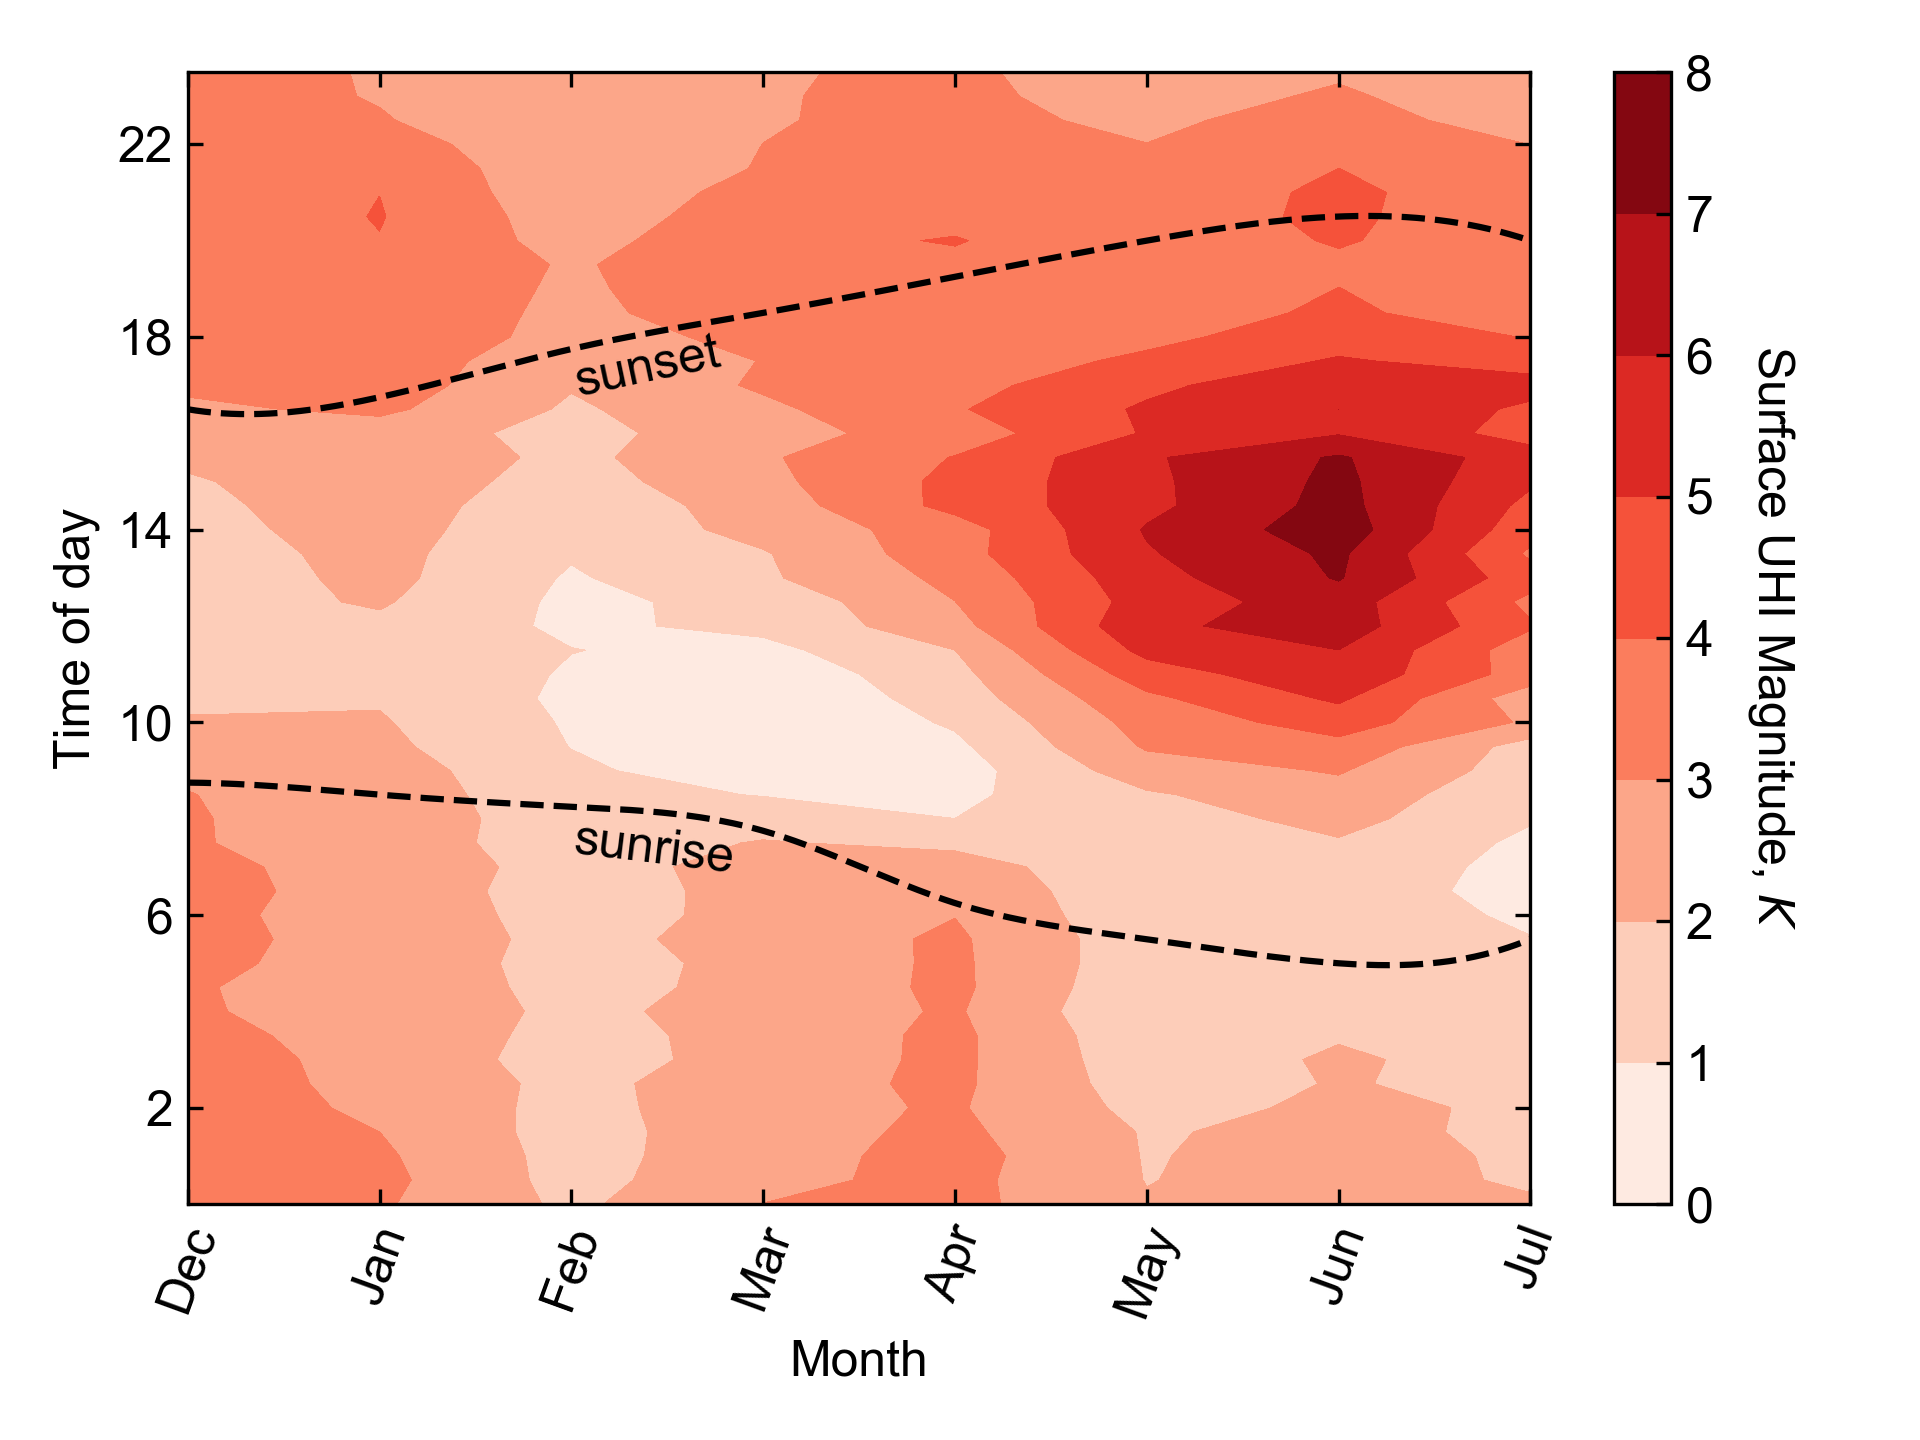
\includegraphics[width=15cm,height=7in,keepaspectratio]{heatsuhi}
	\caption{A heatmap of mean half hourly hemispherical sUHI for each month calculated at 30 \si{\min} intervals for the BUBBLE campaign. Results are interpolated between months.}
	\label{heatsuhi}
\end{figure}

Figure \ref{heatcluhi} shows seasonal variation in diurnal patterns of mean monthly clUHI calculated for the same study period as Figure \ref{heatsuhi}. clUHI development is strongly controlled by the timing of sunset/sunrise cycles and displays the largest seasonal variance in the hours immediately after sunset. Daytime clUHI does not vary significantly across seasons. 

\begin{figure}[H]
	\centering
	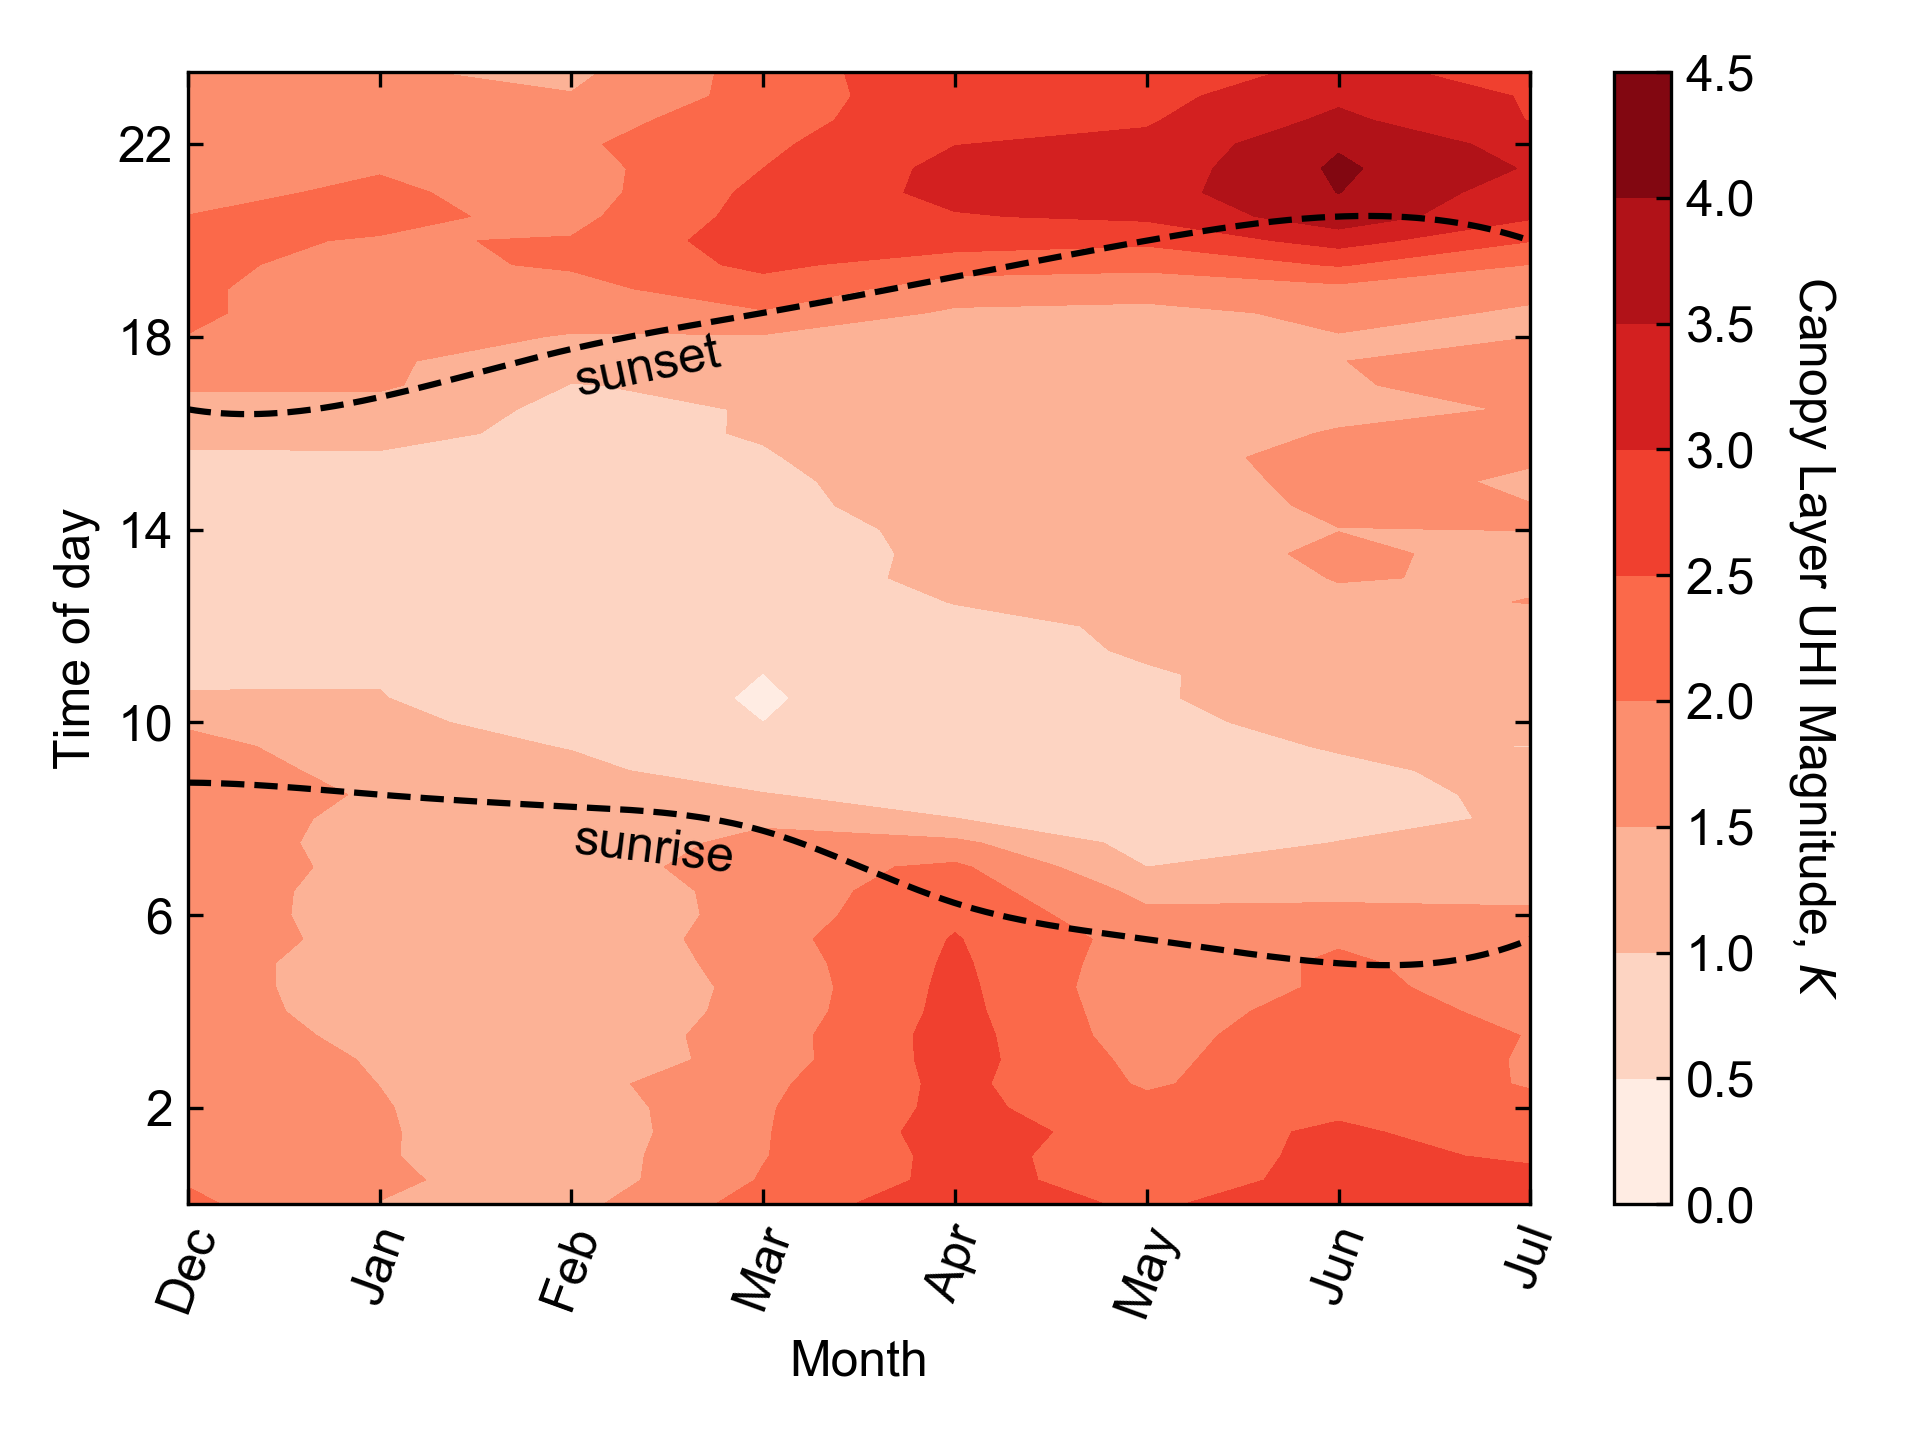
\includegraphics[width=15cm,height=7in,keepaspectratio]{heatatuhi}
	\caption{A heatmap of mean half hourly canopy layer UHI for each month calculated at 30 \si{\min} intervals for the BUBBLE campaign. Results are interpolated between months.}
	\label{heatcluhi}
\end{figure}

Figure \ref{heat_uhi_diff} shows seasonal variation in the difference between mean monthly hemispherical sUHI\textsubscript{norm} and clUHi\textsubscript{norm} for the BUBBLE campaign. By restricting UHI values to a range between one and zero, diurnal patterns of sUHI and clUHI can be compared directly. Comparison of the two in summer shows a peak sUHI approximately two hours after solar noon (when clUHI is small) and peak clUHI approximately two hours after sunset (when sUHI is small). Values near zero in the winder months indicate little variation in both sUHI and clUHI.

\begin{figure}[H]
	\centering
	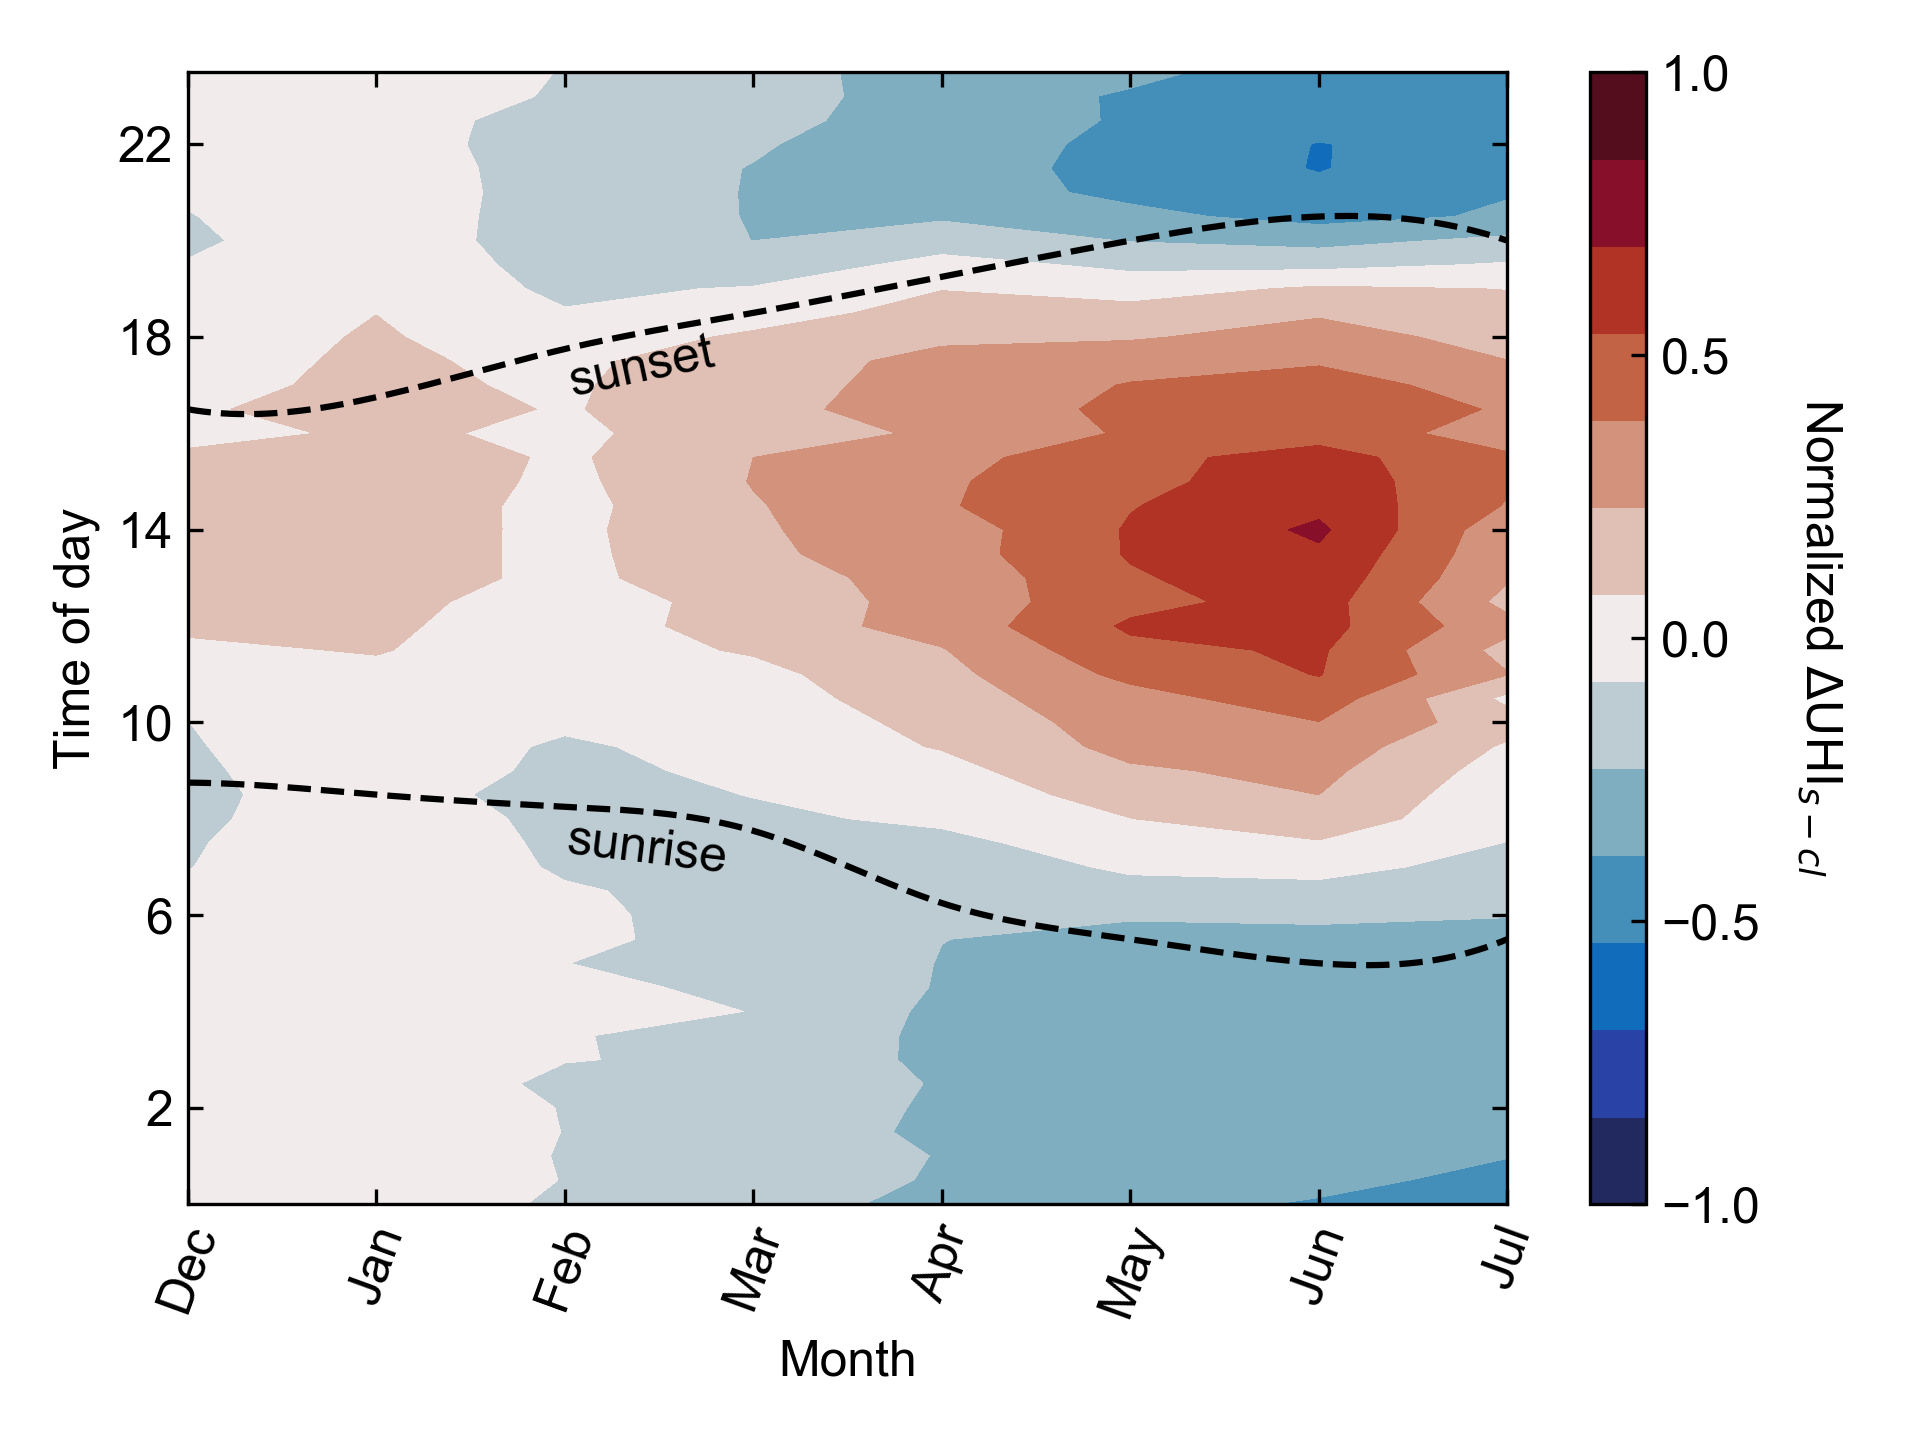
\includegraphics[width=15cm,height=7in,keepaspectratio]{heat_uhi_diff}
	\caption{A heatmap of the difference between mean half hourly hemispherical normalized sUHI and canopy layer UHI for each month calculated at 30 \si{\min} intervals over the BUBBLE campaign. Results are interpolated between months.}
	\label{heat_uhi_diff}
\end{figure}

Figure \ref{vanc_suhi} shows seasonal variations in diurnal patterns of mean monthly hemispherical sUHI magnitudes at 30 minute intervals for the EPiCC campaign. The sUHI in Vancouver shows similar seasonal and diurnal patterns to the sUHI in Basel, but does not persist as far into the late evening hours.

\begin{figure}[H]
	\centering
	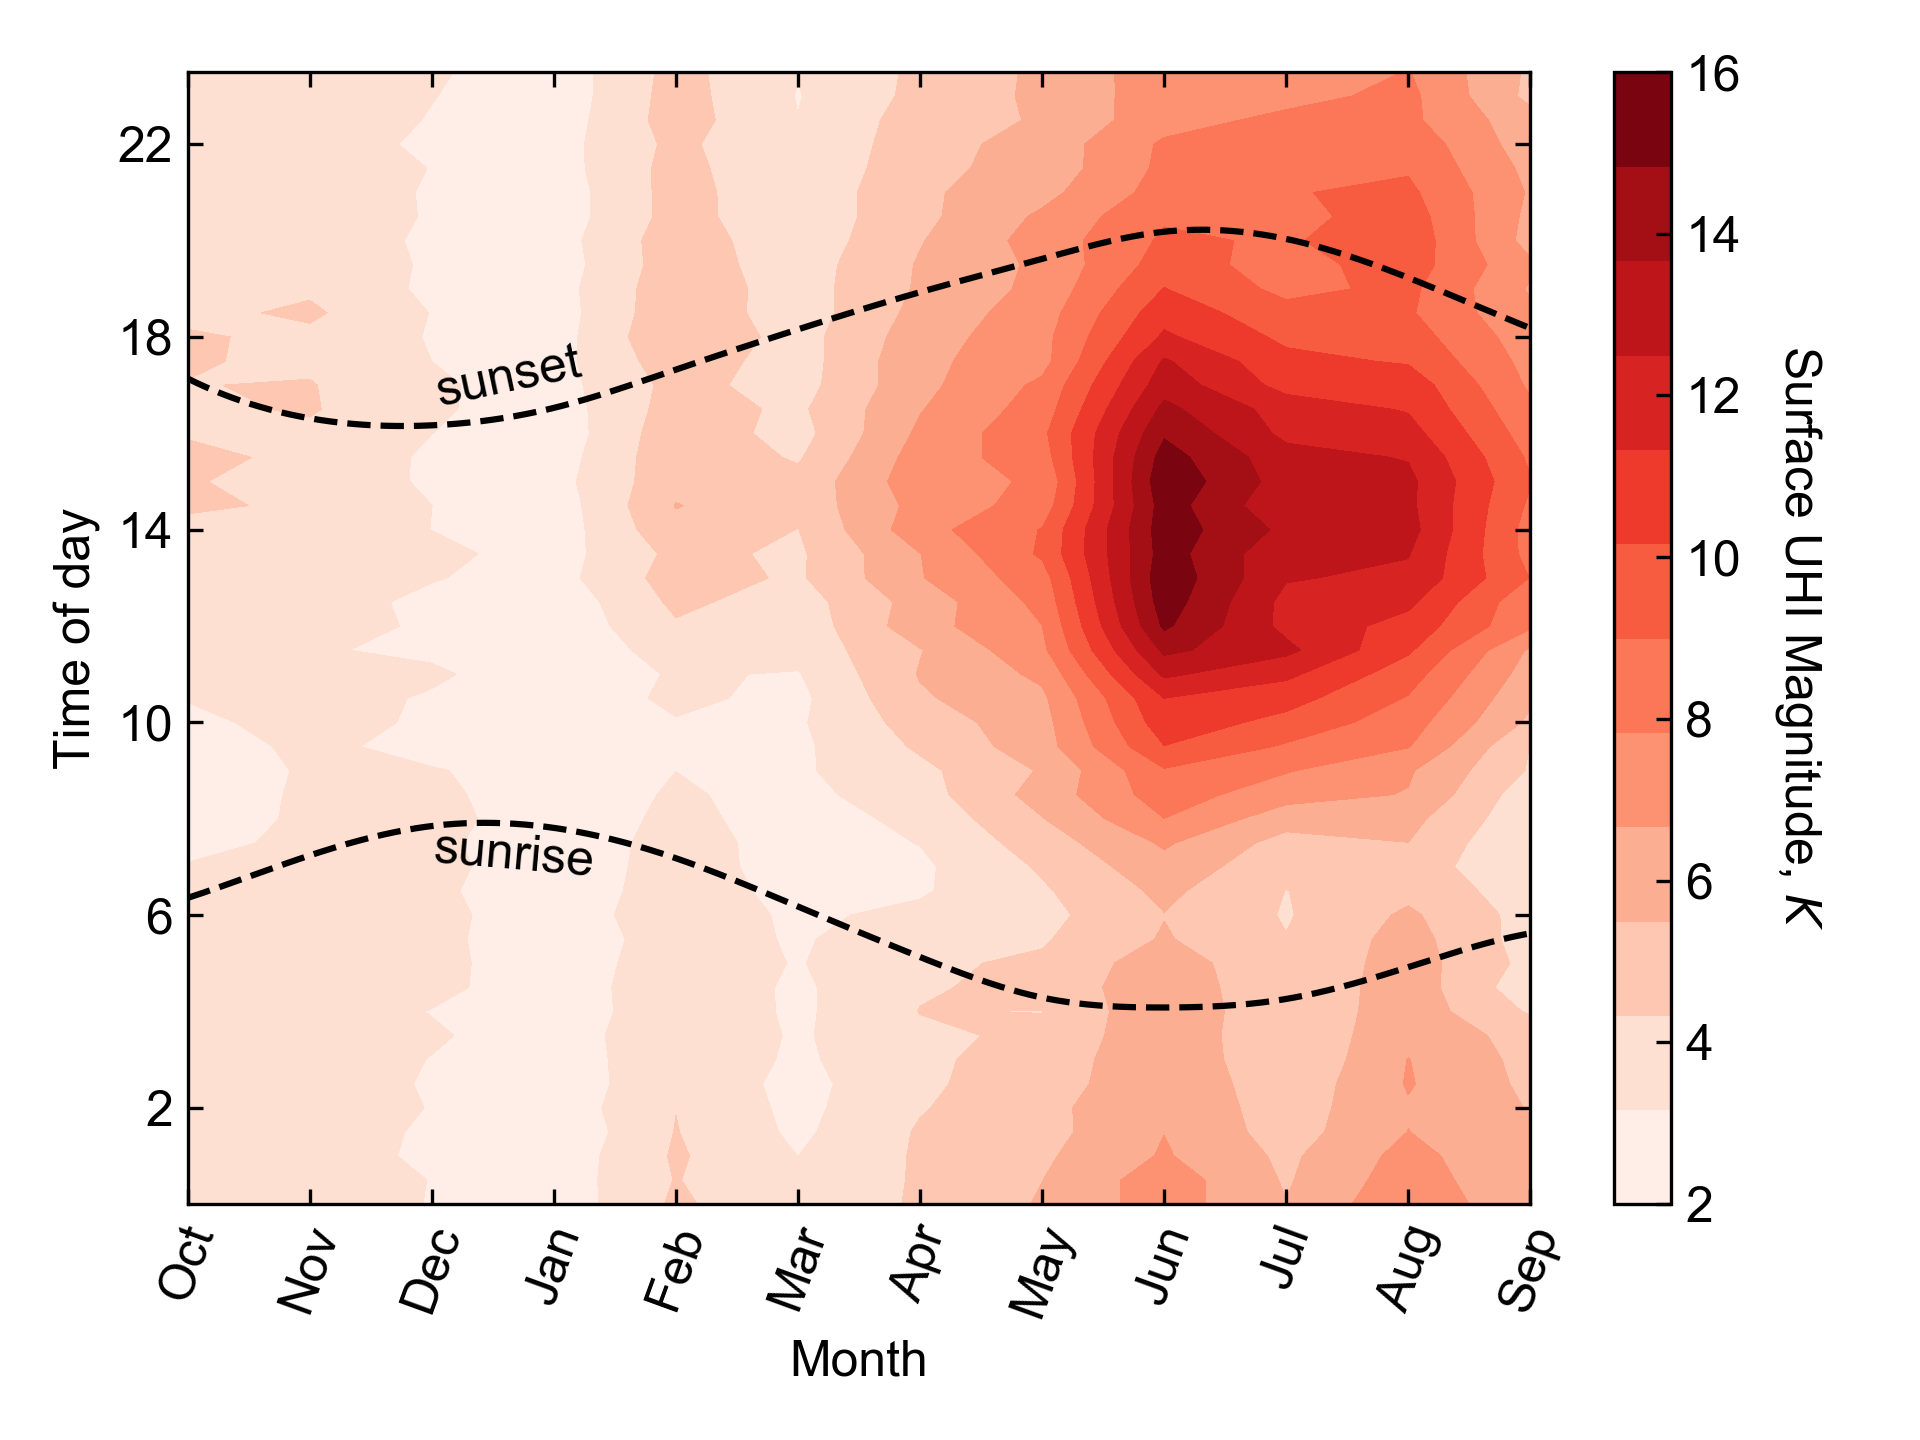
\includegraphics[width=15cm,height=7in,keepaspectratio]{vanc_suhi}
	\caption{A heatmap of mean half hourly hemispherical sUHI for each month calculated at 30 \si{\min} intervals for a year-long subset of the EPiCC campaign. Results are interpolated between months.}
	\label{vanc_suhi}
\end{figure}

Figure \ref{bxsUHI_season_bubble} shows hemispherical sUHI magnitudes for the eight month BUBBLE campaign and binned for winter (December through February) and summer (April through July) seasons. Diurnal variability in sUHI magnitudes is concentrated in summer months, as well as seasonal sUHI\textsubscript{max}. 

\begin{figure}[H]
	\centering
	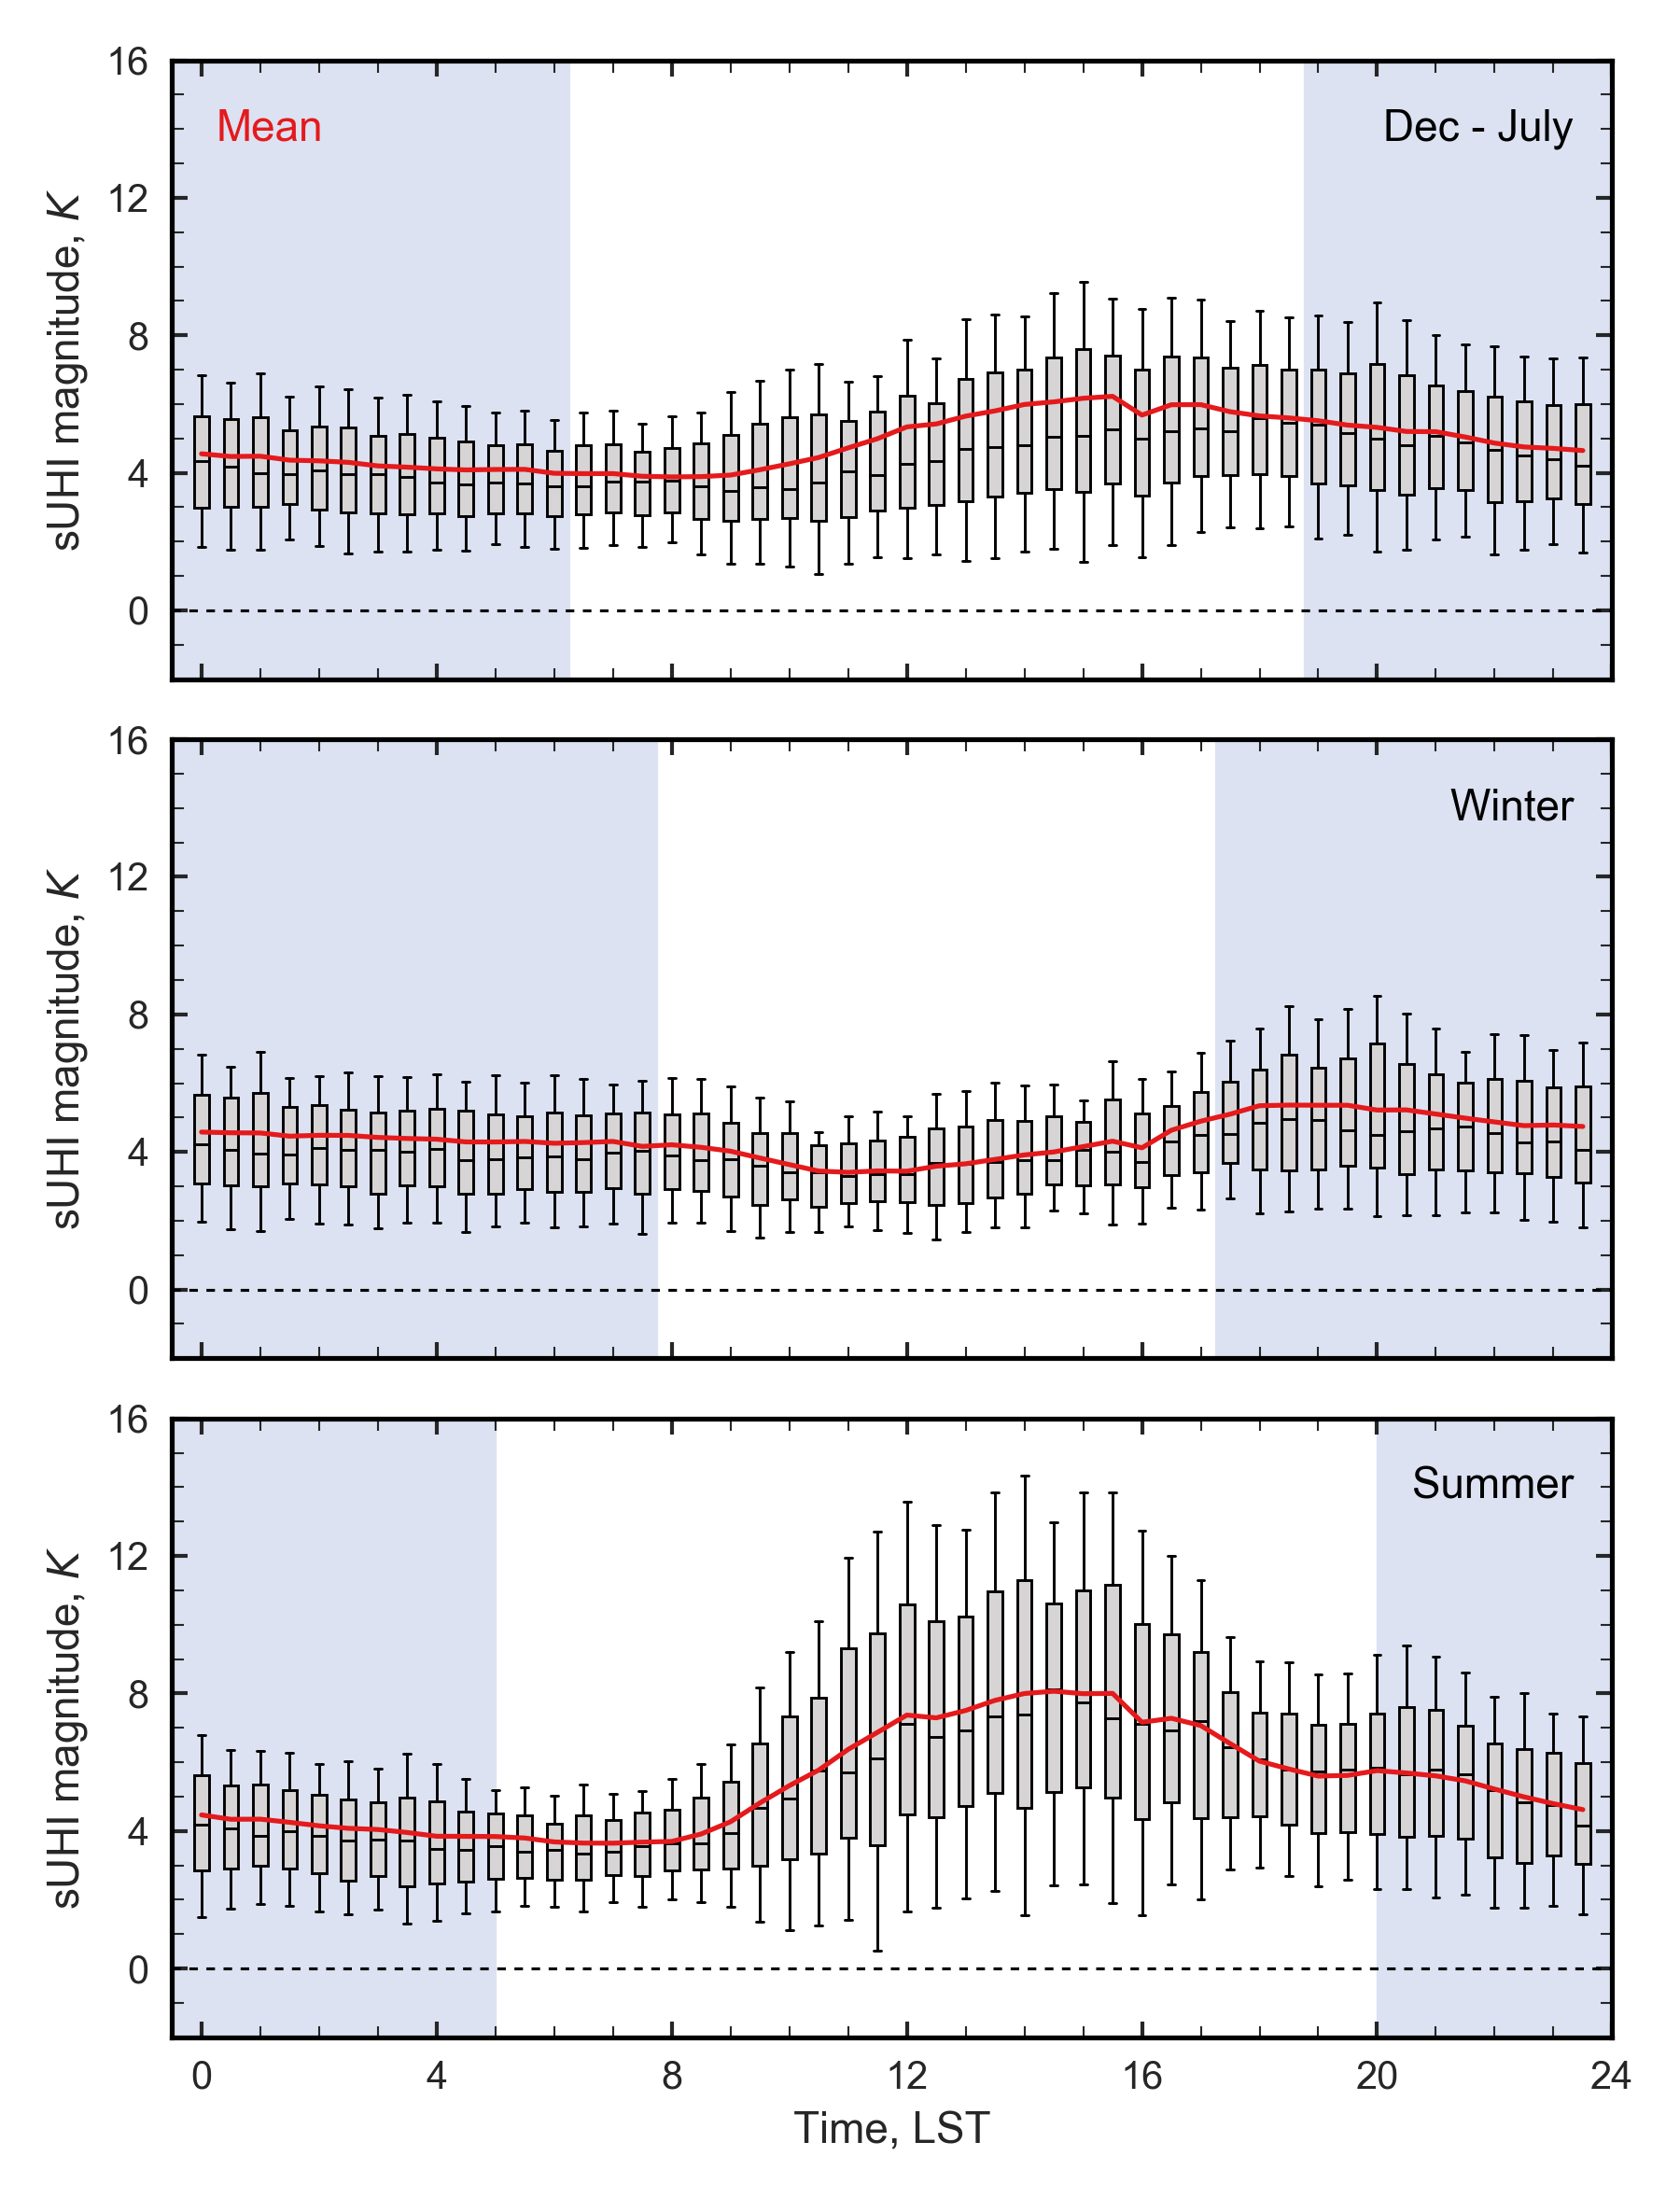
\includegraphics[width=15cm,height=7in,keepaspectratio]{bxsUHI_season_bubble}
	\caption{Hemispherical sUHI magnitudes for the eight month BUBBLE climatology (top) and binned for winter (middle) and summer (bottom) seasons. Grey shading indicates nighttime hours averaged over the bin interval.}
	\label{bxsUHI_season_bubble}
\end{figure}

\subsection{The effect of sensor-surface geometry on sUHI}

Figure \ref{bx_suhi_compare} shows sUHI magnitudes calculated from urban T\textsubscript{comp}, T\textsubscript{plan}, and T\textsubscript{hem}. Compared to sUHI viewed from a complete representation of the urban surface (sUHI\textsubscript{comp}); nadir (sUHI\textsubscript{nadir}) and hemispherical (sUHI\textsubscript{hem}) views of the surface overestimate sUHI\textsubscript{comp} by day and underestimate sUHI\textsubscript{comp} by night. sUHI\textsubscript{nadir} from a nadir view shows the greatest diurnal range of magnitudes, particularly under clear sky 'satellite friendly' conditions. 

\begin{figure}[H]
	\centering
	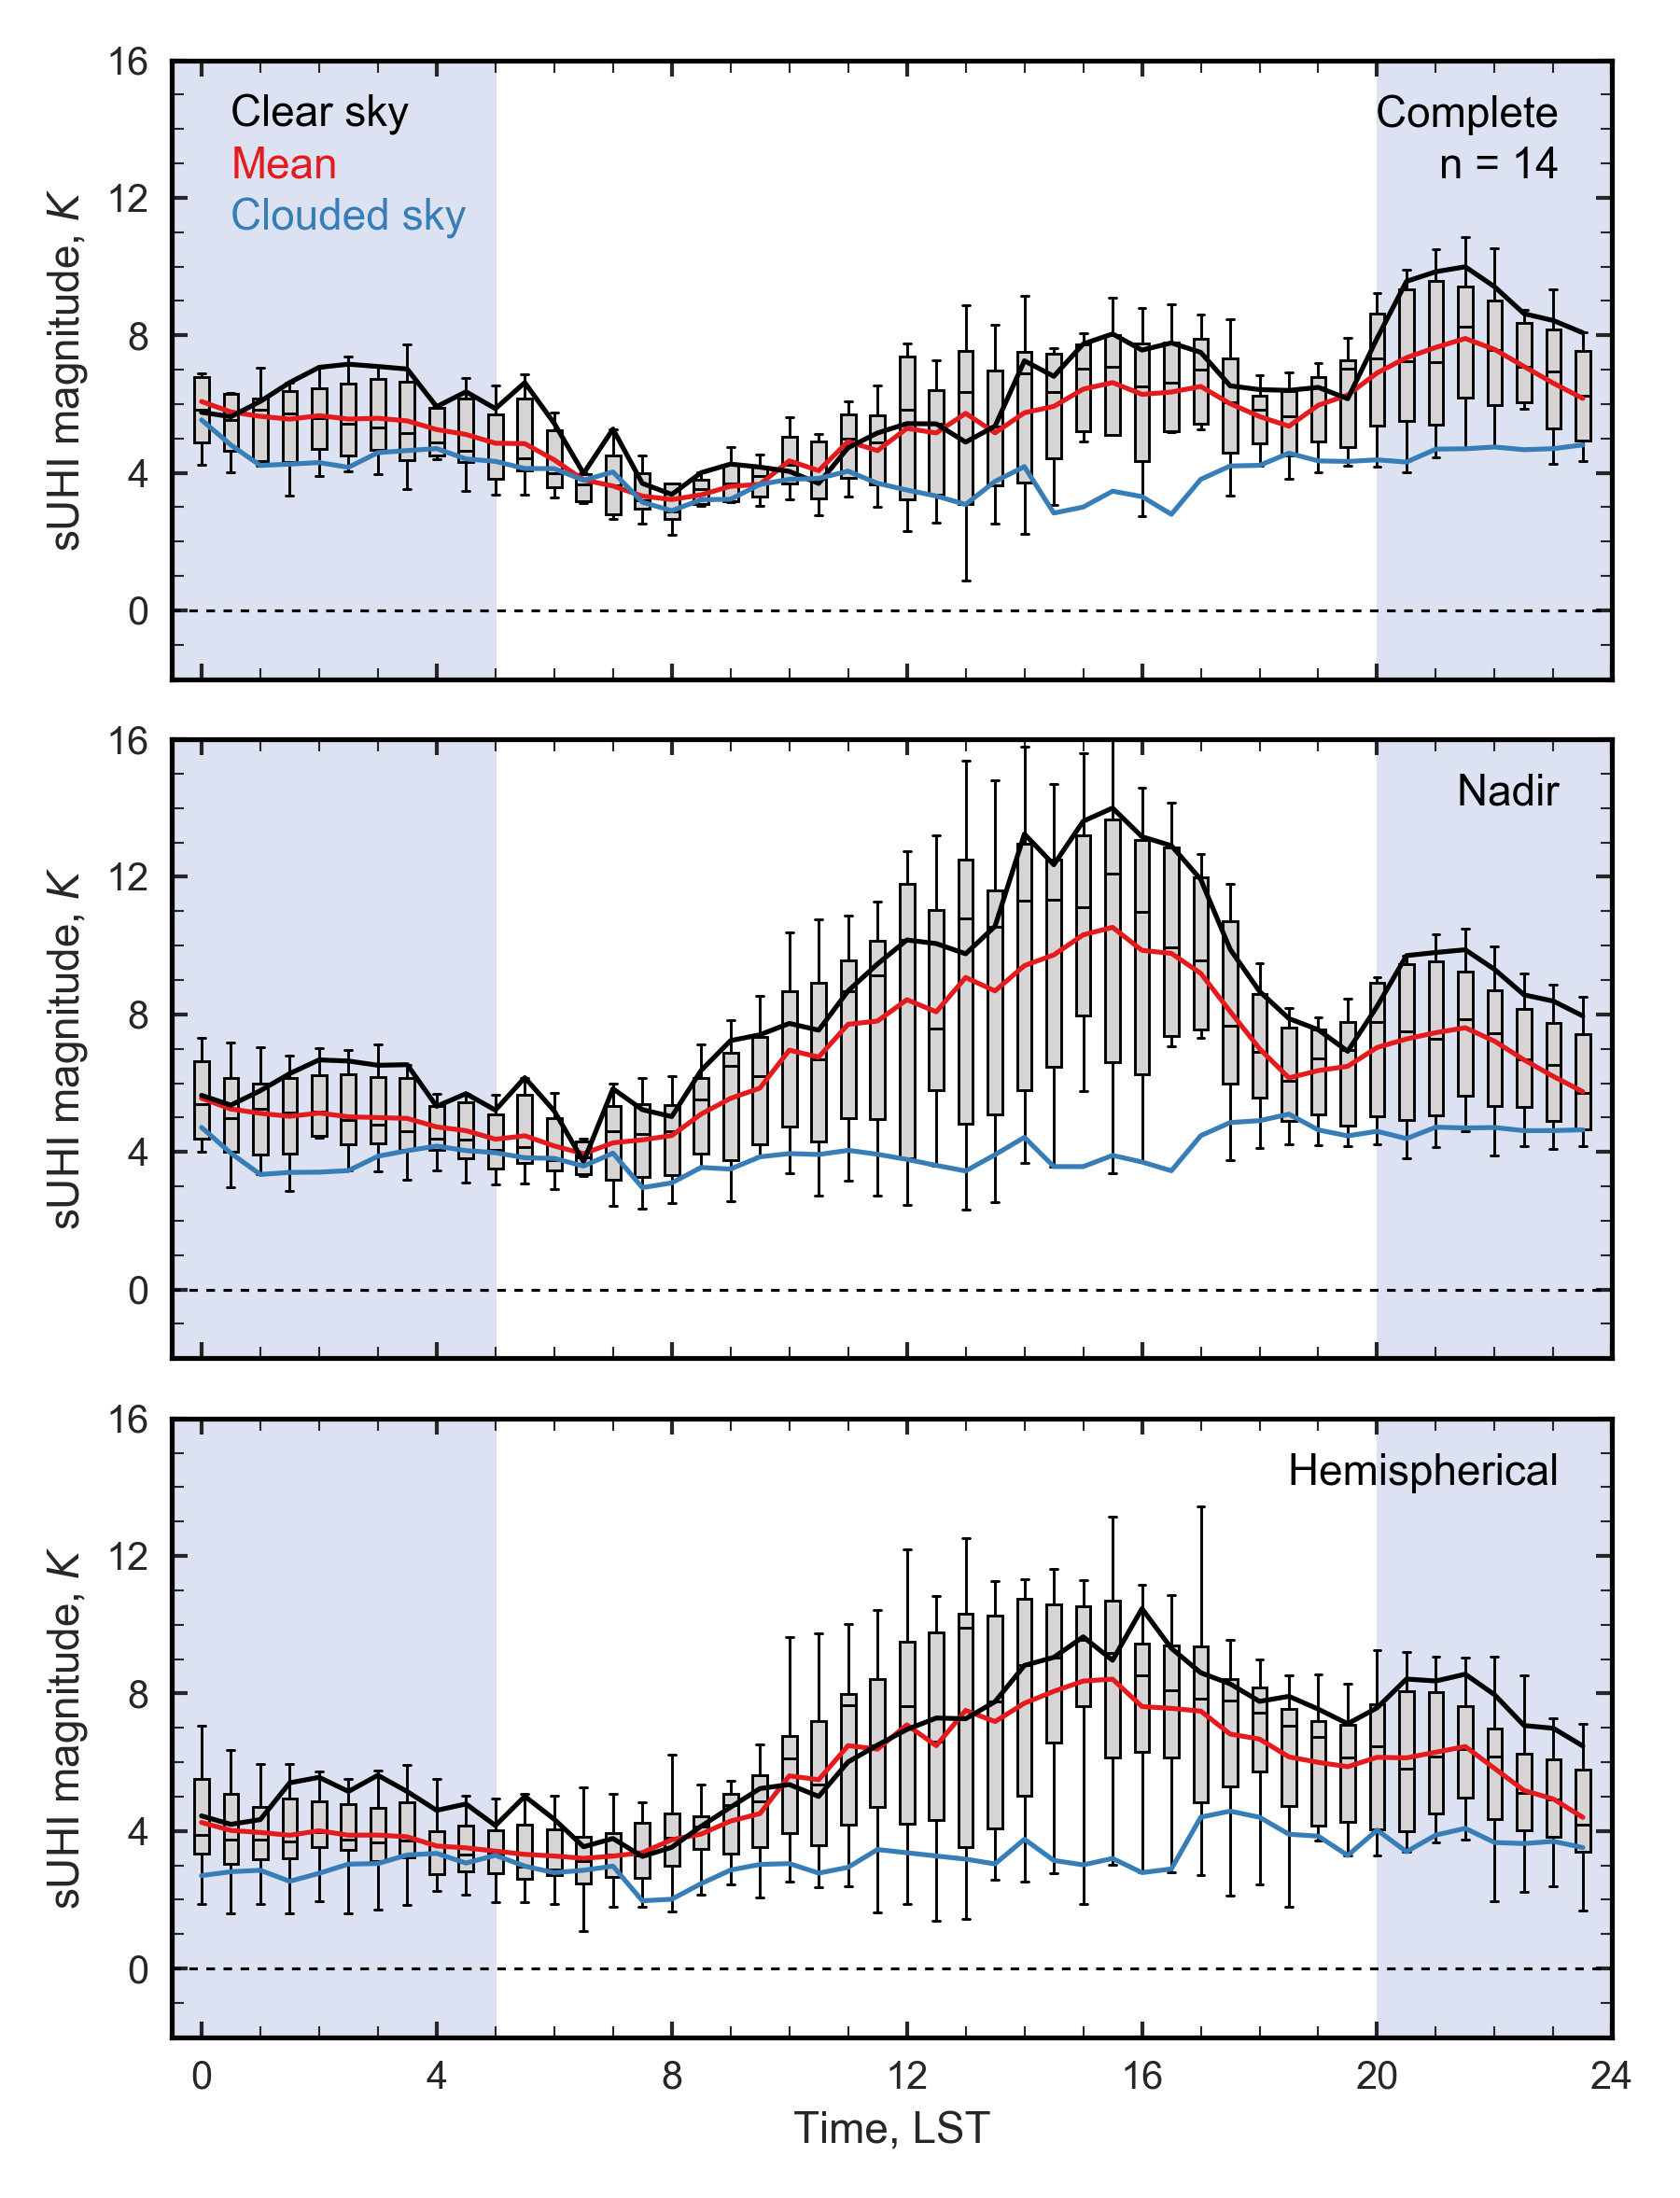
\includegraphics[width=15cm,height=7in,keepaspectratio]{bxsUHI_iop_bubble}
	\caption{A comparison of sUHI magnitudes from complete (sUHI\textsubscript{comp}), hemispherical (sUHI\textsubscript{hem}), and nadir (sUHI\textsubscript{nadir}) remote sensed representations of the Sperrstrasse canyon over the IOP. Each plot includes mean sUHI, as well case days representing sUHI under clear sky and clouded sky conditions.}
	\label{bx_suhi_compare}
\end{figure}

\subsection{The effect of meteorological conditions on sUHI}

Figure \ref{meteo_wv_sol} panel (a) shows mean and maximum sUHI magnitudes as a function of solar radiant exposure over each day of the summer months of the BUBBLE campaign. Point shading indicates the month (white is April and black is July). A clear positive relationship is observed between accumulated solar radiation and both sUHI\textsubscript{max} and sUHI\textsubscript{mean}. Panel (b) of Figure \ref{meteo_wv_sol} shows mean and maximum hemispherical sUHI magnitudes as a function of mean wind velocity for the duration of the eight month BUBBLE climatology. Colors indicate solar radiant exposure accumulated over each day. Similar results are observed when rural winds are substituted.

Figures \ref{meteo_hum} and \ref{meteo_atuhi} show hemispherical sUHI magnitudes as a function of water vapor content and clUHI measured over the BUBBLE campaign. Winter hours are omitted in both as sUHI is small and displays minimal variation in winter. Jamie: still working on getting color palettes for these. Will merge into one figure. 

\begin{figure}[H]
	\centering
	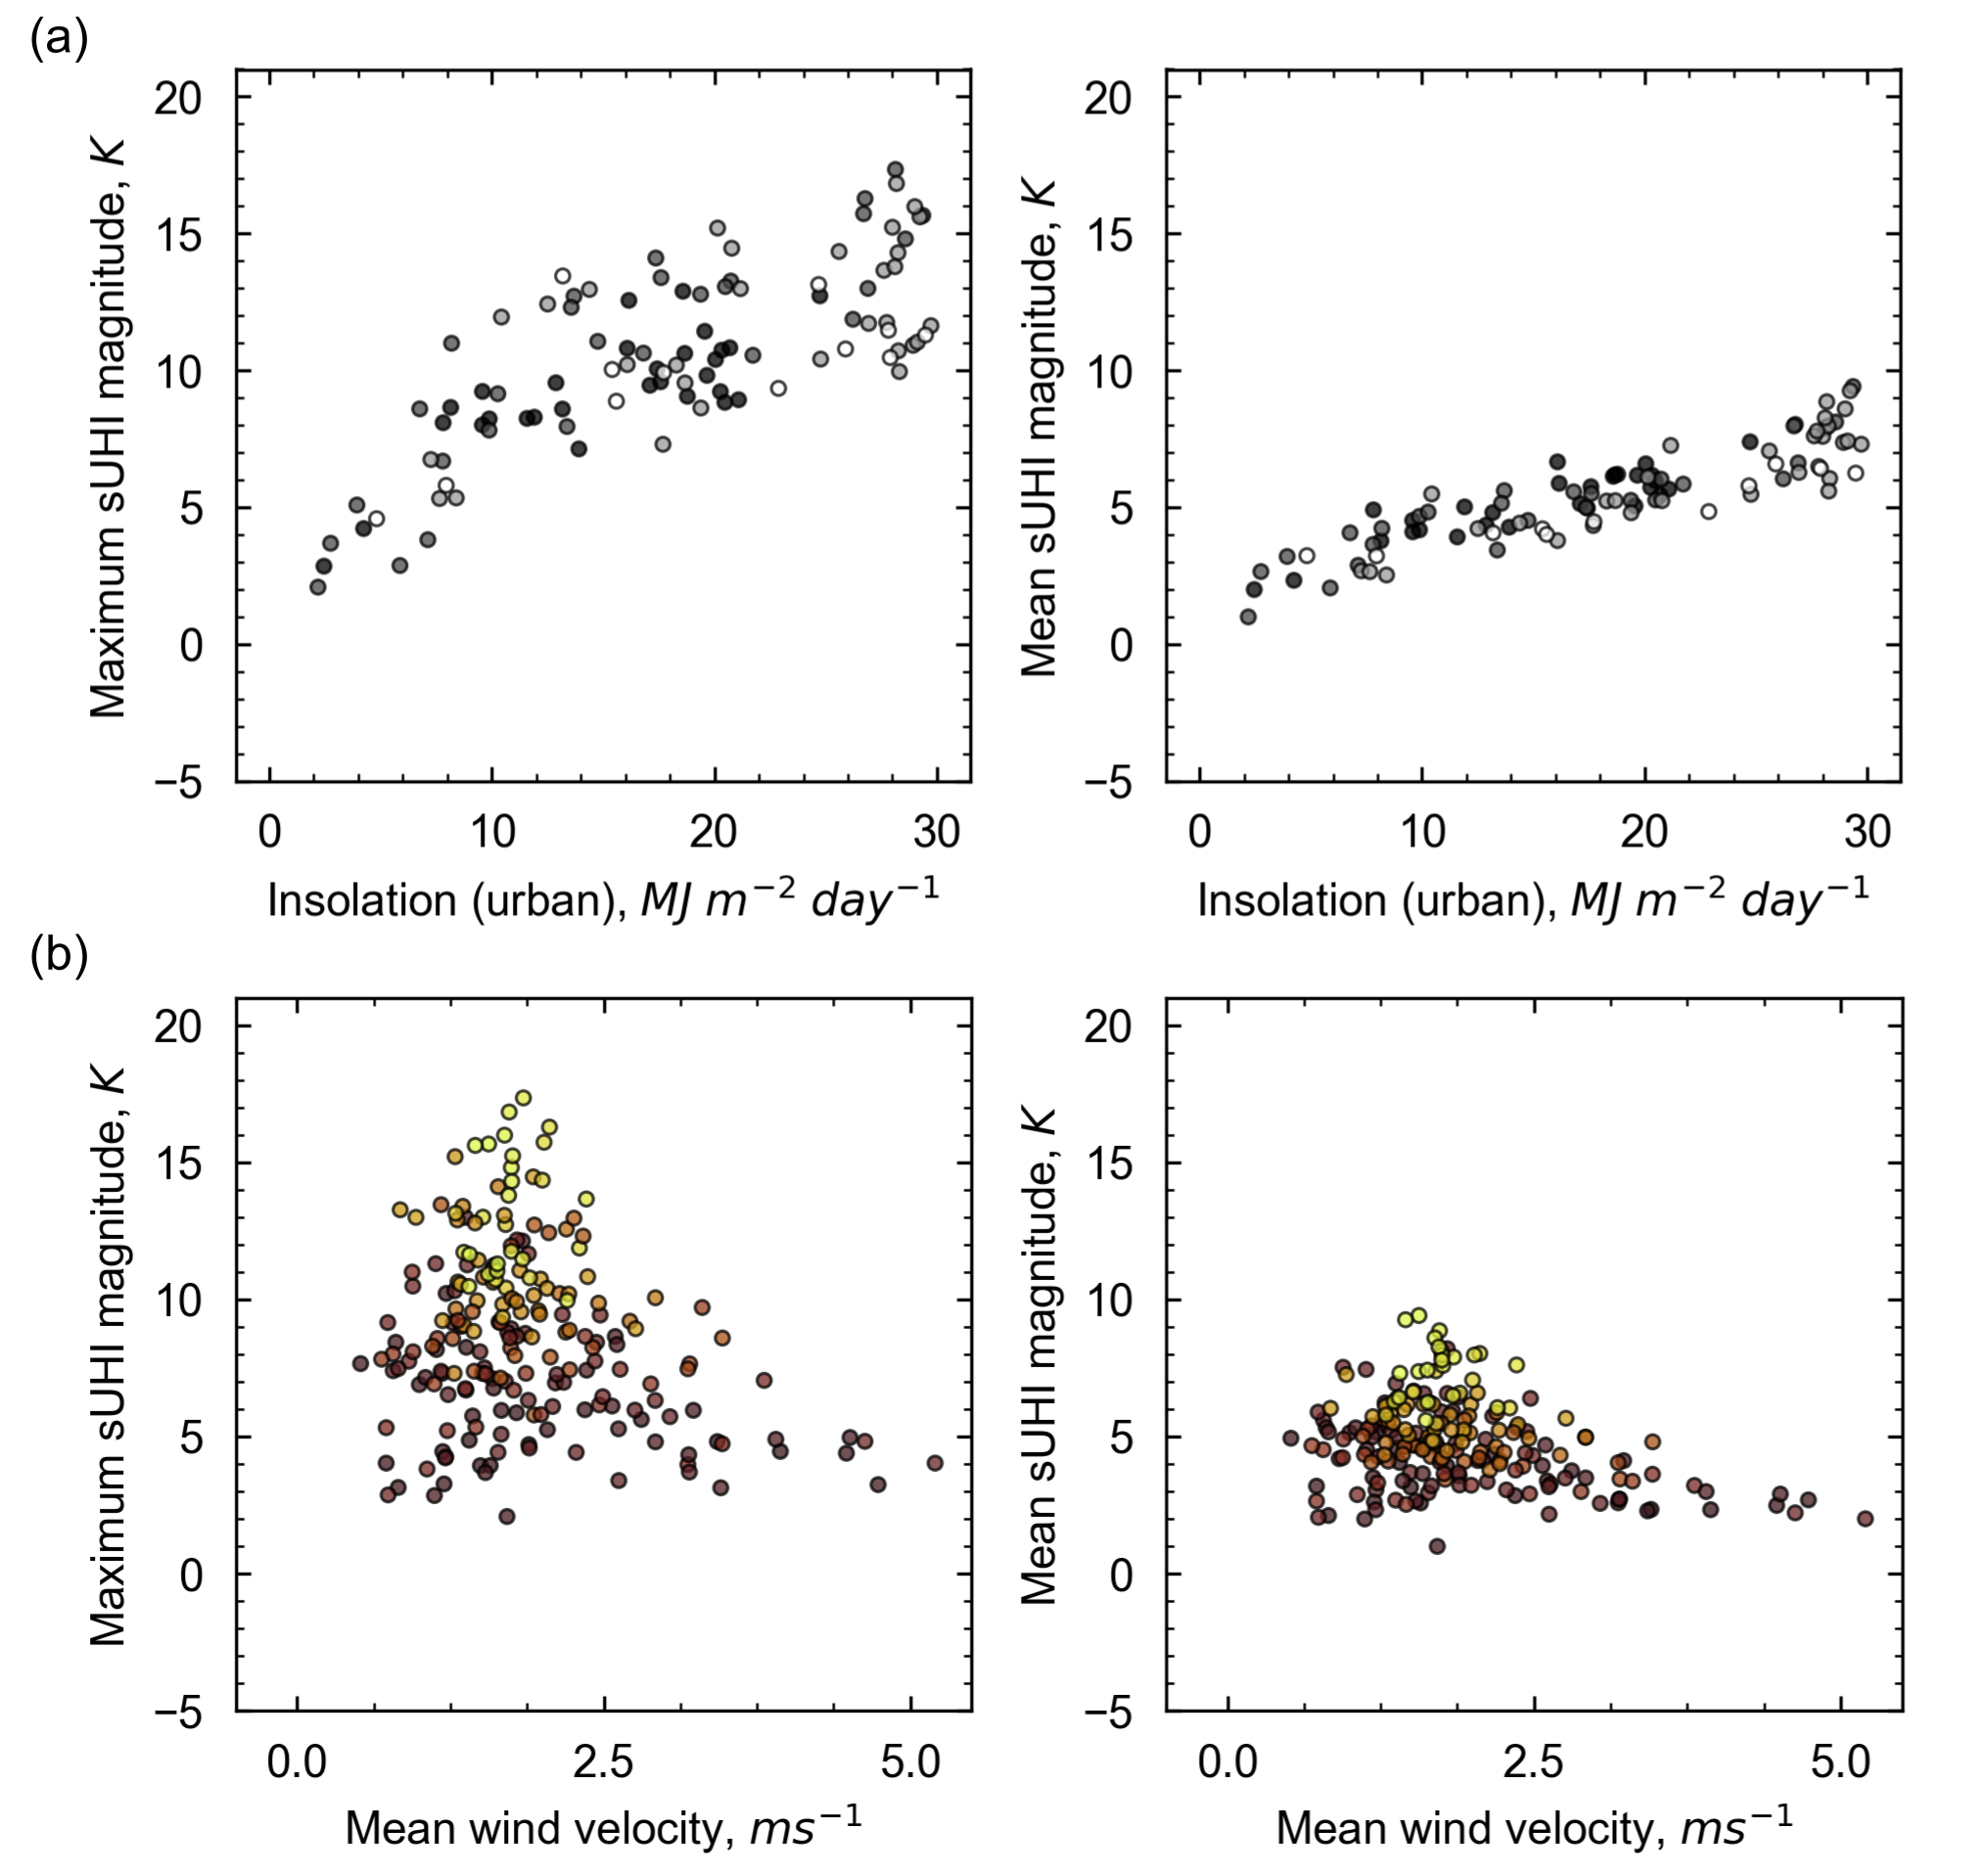
\includegraphics[width=15cm,height=7in,keepaspectratio]{meteo_wv_sol}
	\caption{(a) Maximum and mean 24 \si{\hour} hemispherical sUHI magnitude for each day of April through July versus integrated solar radiant exposure measured over the same 24 \si{\hour} period. Shading indicates month of the year, with dark points indicating later months. (b) Maximum and mean 24 \si{\hour} hemispherical sUHI magnitude for each day in the eight month climatology versus mean wind velocity measured at approximately 2 \si{\meter} above ground at the Sperrstrasse site. Coloring indicates integrated solar radiant exposure over each day.}
	\label{meteo_wv_sol}
\end{figure}

\begin{figure}[H]
	\centering
	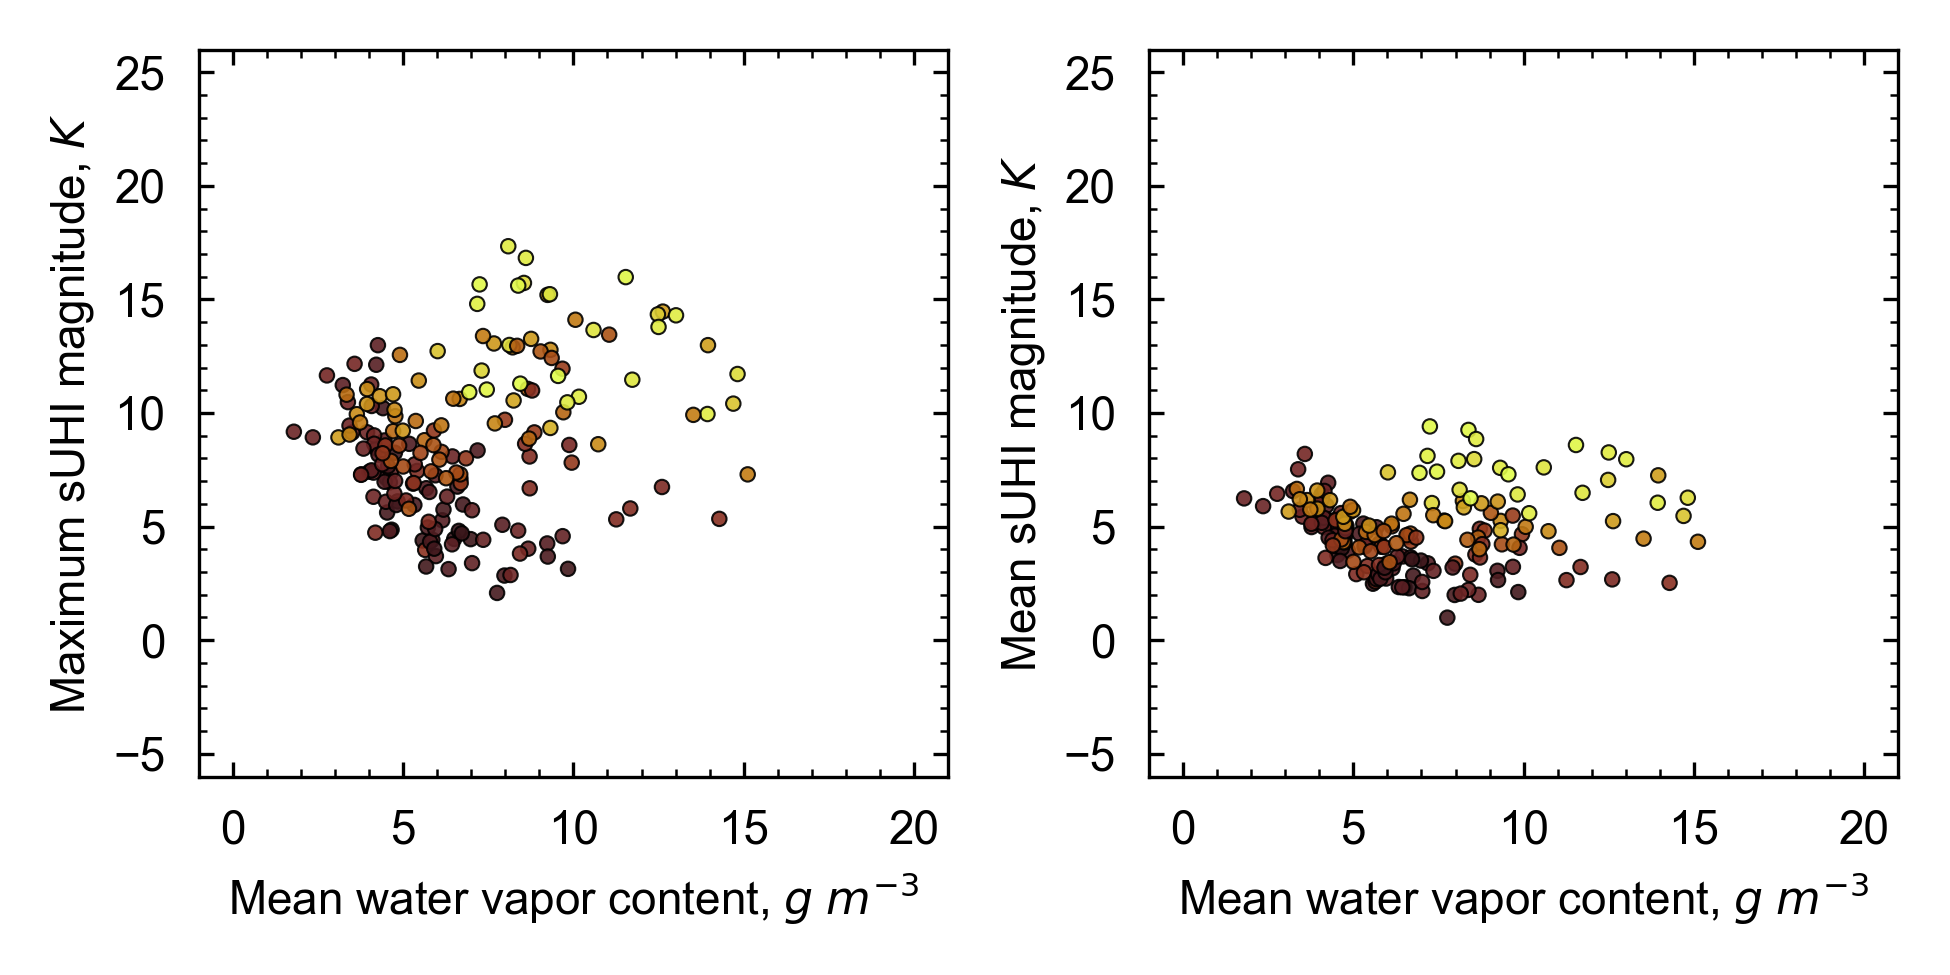
\includegraphics[width=15cm,height=7in,keepaspectratio]{meteo_hum}
	\caption{sUHI magnitude versus atmospheric water vapor content measured at 2 \si{\meter} at the Sperrstrasse site. Similar patterns are observed when rural water vapor content is substituted.}
	\label{meteo_hum}
\end{figure}

\begin{figure}[H]
	\centering
	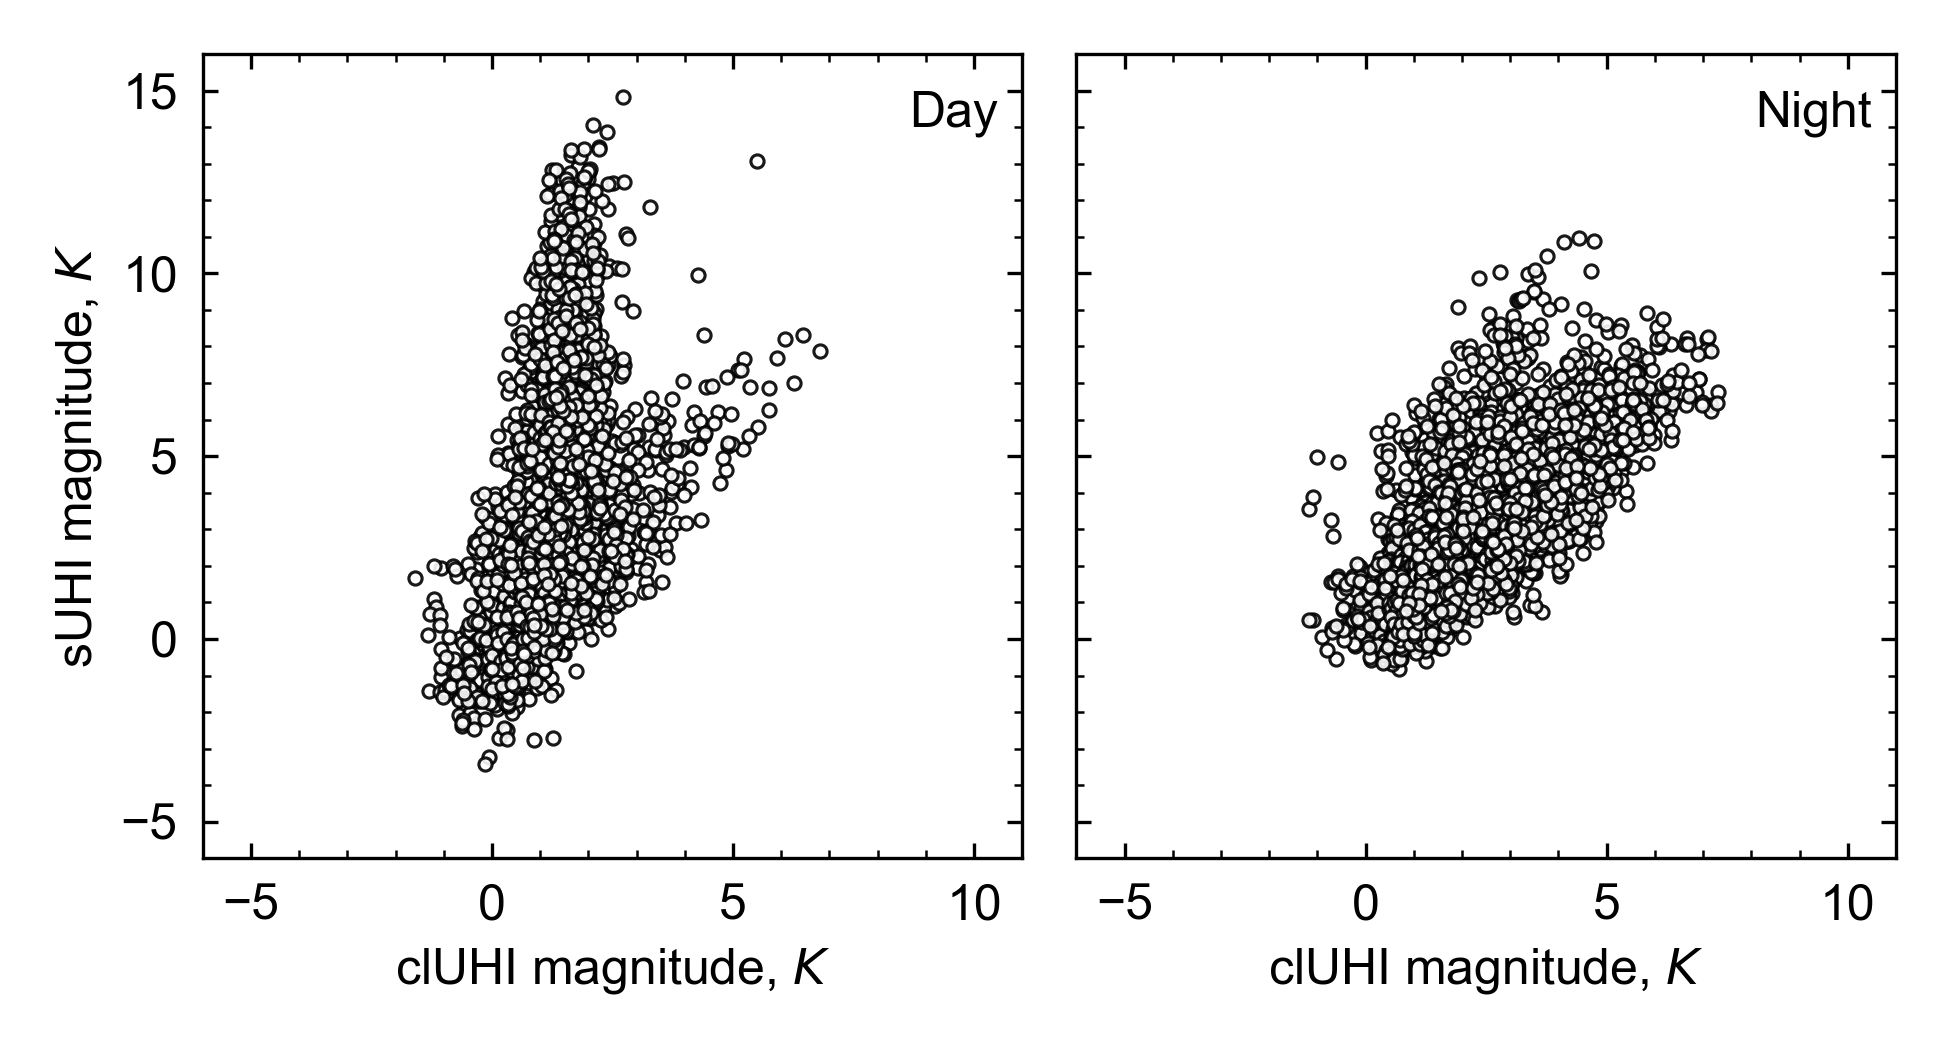
\includegraphics[width=15cm,height=7in,keepaspectratio]{meteo_atuhi}
	\caption{sUHI magnitude versus clUHI magnitude. clUHI is calculated as the difference between urban and rural T\textsubscript{air} measured at 2 \si{\meter} above ground level.}
	\label{meteo_atuhi}
\end{figure}

\pagebreak

\subsection{The effect of rural/non-urban characteristics on sUHI}

Figure \ref{rur_uhi_means} shows urban T\textsubscript{hem, r} from the Sperrstrasse site and rural T\textsubscript{hem, b} for the Lange Erlen and Village Neuf sites as well as their associated hemispherical sUHI magnitudes for a representative, summertime clear sky day. In addition, the figure shows mean normalized hemispherical sUHI and T\textsubscript{hem, b} (calculated from maximum sUHI and T\textsubscript{hem, b} values for each day) for the Lange Erlen and Village Neuf stations. Days were chosen to represent a wide range of summertime conditions and cloud coverages, however, observations at the Village Neuf site were intermittent and n = 9 only applies to hours after 12:00 LST when data could be continuously sampled.

\begin{figure}[H]
	\centering
	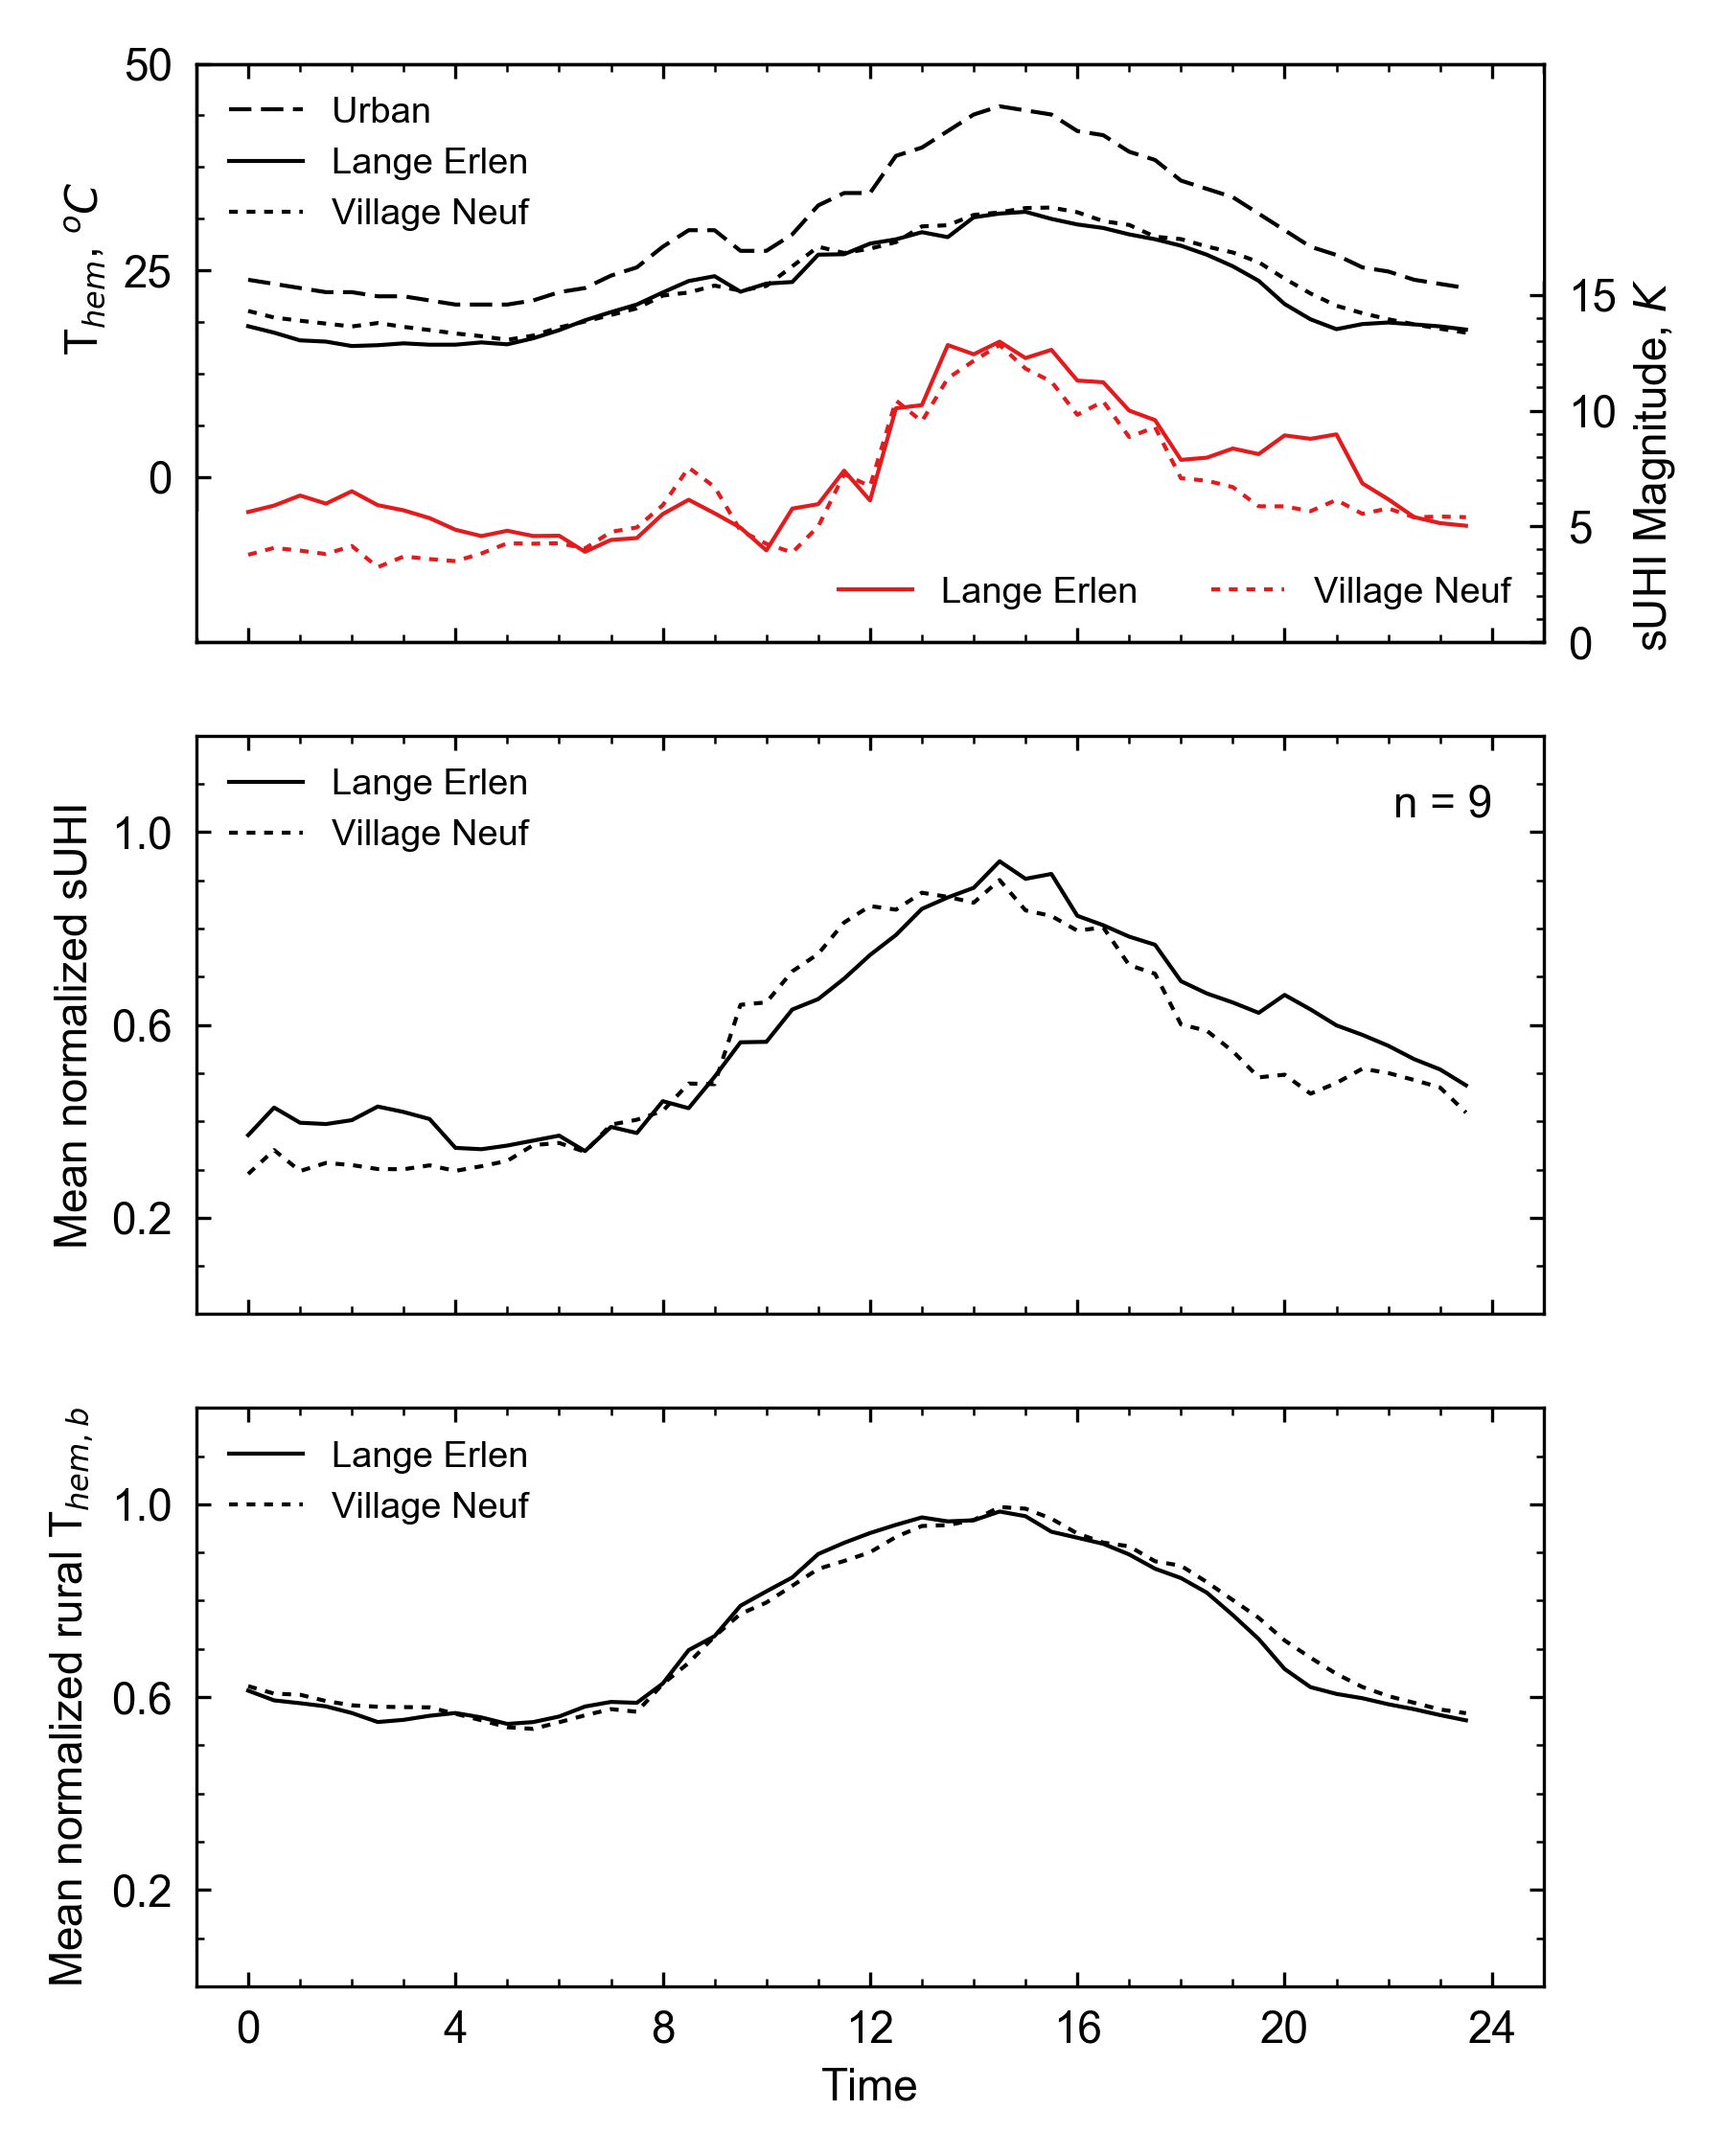
\includegraphics[width=15cm,height=7in,keepaspectratio]{rur_uhi_means1}
	\caption{Top: T\textsubscript{hem} from the Sperrstrasse urban and Lange Erlen and Village Neuf sites and sUHI magnitudes calculated from the two rural stations for a representative summer clear sky day. Middle and bottom: Mean normalized hemispherical sUHI and T\textsubscript{hem, b} calculated for the Lange Erlen and Village Neuf sites. Data at Village Neuf before noon were intermittent, thus n = 9 only applies to values after 12:00 LST. Both sites are sampled over the same truncated period on days with incomplete data.}
	\label{rur_uhi_means}
\end{figure}

\section{Discussion}
\citet{Oke2017} presents a generalized conceptual model for sUHI development for multiple representations of the surface. However, the results in \citet{Oke2017} are based on simulations of an idealized urban area without trees, complex non-orthogonal surface geometry, or sloped facets and have not been supported observationally. The results in this chapter provide an ideal platform to test conceptual understanding of sUHI development, to understand the diurnal and seasonal nature of sUHI and the meteorological factors that drive its development.

\subsection{Diurnal patterns of sUHI}
\label{gen}

sUHI development is the result of urban modification to surface geometry and thermal and radiative properties, most notably sky-view-factor, impervious surface fraction, and thermal admittance (and by relation, urban-rural soil moisture contrasts). These differences alter urban heating/cooling rates relative to non-urban spaces and provide the genesis for diurnal sUHI development. In the early morning hours, rural surfaces respond quickly to insolation at low solar angles, and rural T\textsubscript{surf} rapidly increases. In contrast, shading by urban features causes urban T\textsubscript{surf} to respond more slowly, resulting in a small sUHI\textsubscript{min} in the hours just after sunrise. This is observed in Basel across all representations of urban T\textsubscript{surf} at similar magnitudes. Through the late morning hours, urban heating rates increase relative to rural rates as the solar angle increases and low thermal admittance facets (particularly rooftops) experience more direct insolation and quickly heat up. Increases in urban T\textsubscript{surf} are amplified by the abundance of impervious surfaces, which result in a smaller fraction of insolation partitioned to latent heat relative to vegetated non urban spaces. After the initial spike in rural heating in the early morning hours, urban heating rates overtake rural approximately three to four hours after sunrise and the sUHI slowly grows through midday to a peak at approximately two to three hours hours after solar noon. In the hours after UHI\textsubscript{max}, the solar angle decreases and both urban and rural heating rates decline and begin to converge, as shading by canyon geometry causes some facets to begin to cool.

In the afternoon hours, both urban and rural surfaces transition to cooling, this can lead to several different patterns in evening sUHI development and is strongly controlled by urban surface structure. Relative to non-urban spaces, cooling rates for wall and road facets lag slightly as a result of canyon radiation trapping, this is offset by increased cooling rates for low thermal admittance rooftop facets. These two factors control whether sUHI grows or shrinks in the hours after sUHI\textsubscript{max}. In urban areas with relatively unobstructed sky-view-factors or large rooftop plan area fractions, strong radiative cooling can lead to a sharp reduction in sUHI. The opposite is true of urban areas with restricted sky view factors and tall street canyons with large wall surface area fractions, where canyon radiative trapping reduces radiative cooling and sUHI is maintained through the evening. For the Sperrstrasse canyon, the combination of a narrow but relatively low street canyon results in a slight reduction in Basel's sUHI as strong radiative cooling of rooftops is slightly offset by canyon radiation trapping. The dependence of sUHI development on canyon geometry is illustrated well by comparing nadir and complete representations of sUHI observed in Basel. A nadir view, by virtue of oversampling rapidly cooling rooftops, observes a strong evening decline in sUHI. This is roughly equivalent to sUHI calculated from an urban site with low canyon height to width ratio and a relatively unobstructed sky view factor. In contrast, by sampling vertical facets that cool more gradually, this decline is less evident in sUHI calculated from a complete view of Basel T\textsubscript{surf}. Thus, as expected, remote sensed sUHI analysis is also directionally dependent and subject to anisotropic effects when viewed from a narrow-FOV sensor. These effects not only affect the magnitude of remote sensed sUHI, but may also alter perceived diurnal patterns of sUHI. 
 
After sunset, the unobstructed rural sky-view-factor allows for strong radiative cooling of the surface and rural cooling rates spike relative to urban, leading to a slight jump in sUHI. However, variations in rural thermal admittance, surface geometry, land cover and use, and/or influence from surrounding terrain can result in significant contrasts in rural cooling rates. All of these factors show strong spatiotemporal variation, resulting in large differences in sUHI development depending on rural site characteristics. This is illustrated by two different patterns of post-sunset sUHI development observed for the two rural sites in Basel. Although similar in terms of surface coverage and site geometry, hilly terrain surrounding the Lange Erlen site results in cold air drainage and an increased rural cooling rate, particularly following hot, clear sky days. This effect is not present at the Village Neuf site, where nocturnal cooling rates are likely driven primarily driven by radiative losses. The "extra", largely non-radiative cooling at the Lange Erlen site results in a strong second peak in sUHI that is not present in sUHI calculated using the Village Neuf site. Following site dependent effects on sUHI in the hours after sunset, sUHI in Basel is relatively constant over the nighttime hours, with slight growth observed on clear nights where canyon radiation trapping retards urban nocturnal cooling rates relative to rural. 

% This makes clear the need for proper characterization of the radiative and thermal properties, surface geometry and coverage of rural sites in sUHI analysis, as well as the surrounding topography to ensure characterizations of sUHI development are free of confounding influence. 

%However, has not been observed sUHI in Basel from complete, nadir, and hemispherical representations of T\textsubscript{surf} displays two diurnal peaks, the first in the late afternoon and a second just after sunset. Clear sky conditions amplify this phenomena.Contrasting urban-rural heating rates manifest in  The thermal admittance of many urban surfaces, particularly rooftops, tends to be lower than rural and vegetated environments \citep{Spronken-Smith1998} – particularly in temperate climates where rural soil moisture is largely maintained through summer. Lower urban thermal admittance manifests in a larger diurnal thermal amplitude and greater daytime surface heating. Thus, sensors biased towards low thermal admittance rooftop facets (as is the case with a narrow-FOV sensor and the hemispherical sensor at the Sperrstrasse site), will observe large late afternoon peaks in sUHI, which are not necessarily reflected in sUHI from a complete representation of the surface.

%A second peak in sUHI after sunset is the result of differences in relative cooling rates of urban and rural surfaces. In this case, nighttime sUHI is likely the result of a reduction in urban cooling rates from radiation trapping by canyon walls. However, as is the case with clUHI, post sunset sUHI development is highly dependent on rural site characteristics. Factors such as soil moisture, land cover/use, vegetation types, cold air drainage all result in different after sunset cooling rates (and patterns of sUHI development). These factors can vary significantly over small areas. The second peak sUHI is largest following clear sky conditions when the potential for significant differentials in urban-rural nocturnal cooling rates is maximized. A second peak is observed across all representations of urban T\textsubscript{surf} but is most apparent in complete and nadir representations of sUHI, which, for the Sperrstrasse site, sample T\textsubscript{road} to a greater extent than the hemispherical view. 

%A weak sUHI is maintained through the nighttime as urban and rural cooling rates reach parity in the hours after sunset \citep{Oke2017}. Minimum sUHI is observed just after sunrise, where sUHI magnitudes are occasionally negative. At low solar elevations angles, shading by 3-dimensional urban geometry suppresses heating rates for a large portion of urban surface area, reducing overall urban heating rates in early morning. As the solar elevation angle increases through the morning and more facets experience direct insolation, sUHI develops, with nadir and hemispherical representations displaying more rapid intensification than complete sUHI from a bias towards low thermal admittance and directly sunlit rooftop surfaces.

\subsection{Seasonal patterns of sUHI}

Hemispherical sUHI in both Basel and Vancouver displays significant seasonality, both in terms of its diurnal pattern and overall magnitude. Seasonal variations in sUHI are most evident during the daytime hours, where large seasonal contrasts in cloud cover frequency and solar angle exert strong control on daytime heating rates and sUHI development. Mean monthly sUHI\textsubscript{max} is observed near the summer solstice in both study areas, when days are longest and insolation on clear sky days is most intense, forcing significant contrasts in urban-rural heating/cooling rates and the development of a strong sUHI. In winter, lower overall solar input and frequent cloud cover suppress the potential for urban-rural contrasts in heating/cooling rates and weakens wintertime sUHI development. In Basel, wintertime sUHI has a small peak shortly after sunset, when cold air drainage anomalously amplifies rural cooling rates, increasing the sUHI. This small, after-sunset peak in sUHI observed in both summer and winter observations is specific to the Lange Erlen site and is not generalizable. Cooling rates at the Vancouver Westham island rural site are not affected by cold air drainage and, as a result, sUHI does not display two diurnal peaks in summer nor a coherent peak after sunset in winter months. Thus, observations of seasonal variations in hemispherical sUHI in Vancouver are likely highly generalizable to other mid-latitude cities with distinct winter and summer seasons. 

The sUHI and the clUHI have similar micro meteorological genesis, climatic controls, and display similar seasonal variability, albeit concentrated at different times of the day. This is evident when comparing normalized mean monthly hemispherical sUHI and clUHI - where the range of both types of sUHI is restricted to values between zero and one. In winter, low solar input and frequent cloud cover inhibit variability in both sUHI and clUHI and both are of similar normalized magnitudes. In summer, larger solar input fosters contrasts in urban-rural heating and cooling rates and both clUHI and sUHI are most variable, with peak sUHI in the early afternoon clUHI is smallest, and peak clUHI in the hours after sunset when sUHI is relatively low. These results suggest the following generalization: when conditions that foster the formation of strong urban-rural contrasts in T\textsubscript{air} and T\textsubscript{surf} are present (most notably a large solar input), sUHI peaks approximately two hours after solar noon and clUHI peaks approximately two hours after sunset. Thus, a surface urban heat island is not simply a stronger, more pronounced, canopy layer urban heat island. 

\subsection{Sensor-surface-sun geometries and sUHI}

Sensor-surface geometry exerts significant influence on observed sUHI magnitudes. 2-dimensional, complete, and hemispherical observations of sUHI not only yield different magnitudes but also different diurnal sUHI regimes and peak timings. Variations in observed sUHI across different sensor sampling regimes are largest under clear sky, hot conditions, coinciding with typical seasonal and diurnal sUHI\textsubscript{max}. In general, as urban T\textsubscript{surf} is most often viewed from the top down, remote sensors preferentially sample horizontally oriented facets with unobstructed sky view factors and undersample or ignore vertical and sloped facets with more obstructed sky view factors. Over/undersampling of the urban surface changes both the magnitude and character of remote sensed urban T\textsubscript{surf} and sUHI. 

In an analysis of Basel sUHI from complete, nadir, and hemispherical representations of the surface, significant variation in remote sensed sUHI was observed across sensor sampling regimes at all times of the day. Variations in observed sUHI are most evident on clear sky, hot days in the hours after solar noon, when microscale spatiotemporal contrasts in urban T\textsubscript{surf} are largest. Cloud cover suppresses the influence of sensor-surface geometry on remote sensed sUHI by reducing microscale geometric and spatiotemporal contrasts in urban T\textsubscript{surf}, resulting in less facet-scale heterogeneity in urban T\textsubscript{surf} and reducing the overall magnitude of sUHI for all definitions. 

By undersampling vertical and sloped urban surfaces and oversampling low thermal admittance materials, sUHI\textsubscript{nadir} overestimates mean afternoon sUHI\textsubscript{comp} by approximately 3.5 \si{\kelvin} and up to 6.0 \si{\kelvin} under clear sky “satellite friendly” conditions. This constitutes a significant bias in remote sensed sUHI\textsubscript{max} as sUHI\textsubscript{nadir} overestimates the 'true' sUHI\textsubscript{comp} by nearly double under clear sky conditions. As clear sky conditions are the only conditions under which satellite TIR remote sensors can operate, and make up a large fraction of the urban T\textsubscript{surf} literature, these biases are pervasive and cannot be ignored. In contrast to sUHI\textsubscript{nadir}, sUHI\textsubscript{hem} samples the urban surface in 3-dimensions ("seeing" a wider range of facet types and orientations) and yields a much smaller mean daytime overestimation (0.5 \si{\kelvin}), particularly under clear sky conditions (1.0 \si{\kelvin}), providing a significantly more representative depiction of urban T\textsubscript{comp} and sUHI\textsubscript{comp}, in addition to allowing for time-continuous analysis.

\subsection{Meteorological controls on sUHI}

sUHI is highly dependent on meteorological conditions, which account for much of the day to day variation sUHI magnitudes. Conditions that foster the largest microscale spatiotemporal contrasts in urban T\textsubscript{surf} also entail the largest sUHI magnitudes. Contra, conditions that suppress microscale contrasts in T\textsubscript{surf} show reduced sUHI magnitudes. As such, sUHI development is strongly tied to integrated solar radiant exposure accumulated over a day and wind velocity, which display positive and negative relationships with sUHI magnitudes respectively. Meteorological controls on sUHI are summarized in Table \ref{meteo_cont}.

The relationship between solar radiation and sUHI is relatively simple but easily misinterpreted. Surfaces (both urban and otherwise) change in temperature based on accumulated radiative or convective gains or losses - as such, instantaneous changes in insolation have little effect on sUHI magnitudes. Thus, to say that sUHI is a function of measured incoming solar radiation (in \si{\watt\per\square\meter}) does not accurately characterize the relationship and produces a significant amount of unrepresentative scatter. Strong accumulated solar heating of the surface combined with differences in urban and rural thermal properties and sunlit shading geometries fosters the development of large daytime urban-rural contrasts in T\textsubscript{surf} and T\textsubscript{air} and the development of strong sUHI by day and clUHI by night. Thus, sUHI\textsubscript{max} often coincides with insolation\textsubscript{max}. Under cloudy conditions, reduced accumulated solar heating of the surface suppresses the development of urban-rural thermal contrasts, resulting in reduced sUHI magnitudes. Owing to its dependence on accumulated solar heating, $\Delta$T\textsubscript{hem, r - air} has a similar positive effect on sUHI magnitudes. 

Wind velocity has a similarly nuanced relationship with sUHI. Winds affect surface heating and cooling rates by facilitating convective cooling (or, under less common circumstances, convective heating). In general, as wind velocity increases, convective heat losses increase and T\textsubscript{surf} decreases. This suppresses microscale spatiotemporal variations in T\textsubscript{surf} as hot sunlit surfaces experience greater rates of convective cooling under high wind conditions than cooler shaded surfaces. This reduces overall urban and rural T\textsubscript{surf} and inhibits sUHI development. Nighttime sUHI is also affected by wind velocity as the formation of a near surface thermal inversion, which increases radiative cooling in non-urban areas, requires calm winds. As such, increased nighttime wind velocity decreases nocturnal sUHI.

As was found with correction magnitudes in Chapter \ref{paper1}, sUHI magnitudes are not strongly correlated with water vapor content as, in the absence of fog, humidity near the surface does not strongly influence surface heating or cooling rates in and of itself. Atmospheric transmittance of longwave radiation decreases sharply with small increases in water vapor when the atmosphere is very dry - shown in Figure \ref{humtest}. As water vapor content increases from zero, variation in spectral atmospheric transmittance decreases. Therefore, typical variations in urban and rural humidities have little effect on the fraction of outgoing longwave radiation available for heating the canopy layer air volume through absorption and for heating of the surface by atmospheric emission. As a result, water vapor content has little effect on sUHI. 

\begin{table}[H]
	\centering
	\caption{A summary of the relationship between sUHI, meteorological variables, and clUHI.}
	\label{meteo_cont}
	\begin{tabular}{lc}
		\toprule 
		An increase in $x$, has a/an... & $y$ effect on sUHI magnitude. \\
		\midrule
		$\Delta$T\textsubscript{surf - air}, \si{\kelvin} &\textit{increasing} \\
		&\\
		T\textsubscript{surf}, \si{\degreeCelsius}  & \textit{increasing} \\
		&\\
		T\textsubscript{air}, \si{\degreeCelsius} & \textit{increasing} \\
		&\\
		Insolation, \si{\mega\joule\per\meter\squared\per\day} & \textit{increasing}  \\
		& \\
		Water vapor content, \si{\gram\per\meter\squared} & \textit{negligible} \\
		&\\
		Wind velocity, \si{\meter\per\second} &\textit{decreasing} \\
		&\\
		clUHI, \si{\kelvin} &\textit{increasing} \\
		\bottomrule
	\end{tabular} 
\end{table}

clUHI and sUHI develop at different times of day and, thus, have a complex diurnal relationship. By day, variation in clUHI is minimal and shows weak positive correlation with sUHI. Occasionally, under clear sky conditions following hot days, strong evening radiative cooling forces clUHI development slightly before sunset. This causes a slight bifurcation in clUHI versus sUHI. By night, clUHI shows greater variation and a stronger, more positive relationship with sUHI, most evident on clear sky nights when urban-rural contrasts in air and surface cooling rates are strongest. 

\section{Conclusion}

This chapter presents the results of an analysis of two time-continuous long-term climatologies of the surface urban heat island effect in Basel, Switzerland and Vancouver, Canada derived using the method presented in Chapter \ref{paper1}. Hemispherical sUHI magnitudes display significant seasonal and diurnal variation and are largest in summer months during the late afternoon during which solar heating of the surface is most intense, forcing the development of strong urban-rural contrasts in T\textsubscript{surf}. Seasonality in late afternoon sUHI is largely dependent on accumulated radiative exposure over the day which displays a strong positive relationship with sUHI magnitudes. In the winter months, a reduced overall solar input and increased cloud cover frequency suppresses daytime sUHI development resulting in less variability in sUHI, and lower overall sUHI magnitudes. 

Remote sensed sUHI is highly dependent on sensor-surface-sun geometry. This results in significant variation in the character of urban T\textsubscript{surf} and sUHI when observed from sensors with different spatial, geometric, and temporal sampling regimes. Thus, traditional methods for thermal remote sensing of urban areas do not capture the true temporal and geometric nature of the urban effect on land T\textsubscript{surf}. Urban effective anisotropy results in large geometric biases in remote sensing of urban areas as traditional satellite and aerial remote sensors sample only a fraction of the urban surface. These geometric biases manifest not only in deviation between observed sUHI magnitudes and the 'true' complete sUHI, but also impact characterizations of diurnal and seasonal patterns of sUHI and urban T\textsubscript{surf}. Geometric biases in thermal remote sensing of urban area are compounded by myriad temporal biases across a range of temporal scales, as traditional methods for urban thermal remote sensing are not time-continuous and only operable under clear sky conditions. Both geometric and temporal biases affect the vast majority of sUHI study, most of which is performed using only a small number of satellite remote sensors, to which these biases are inherent.

This study provides the first, long-term, temporally continuous, geometrically representative analysis of urban T\textsubscript{surf} and sUHI. By sampling the urban surface in 3-dimensions and time-continuously, the method utilized in this chapter overcomes and quantifies spatial and temporal biases in the satellite thermal remote sensing record to better understand the geometric and temporal effects of a city on the surface climate. Further application of the method in other urban areas can help to facilitate a better understanding of the true nature of sUHI across myriad time scales and help to quantify the magnitude of geometric and temporal biases inherent in the satellite sUHI record.

\cleardoublepage 
\phantomsection  
\renewcommand*{\bibname}{References}
\addcontentsline{toc}{section}{\textbf{References}}


\putbib
\end{bibunit}